\documentclass[11pt,a4paper,faculty=we,language=en,doctype=report]{cls/ugent-doc}

% Optional: margins and spacing
%-------------------------------
% Uncomment and adjust to change the default values set by the template
% Note: the defaults are suggested values by Ghent University
%\geometry{bottom=2.5cm,top=2.5cm,left=3cm,right=2cm} 
%\renewcommand{\baselinestretch}{1.15} % line spacing
\setlength{\headheight}{13.59999pt}

% Python code
%---------------------------------------------
\usepackage{tcolorbox}
\tcbuselibrary{minted,breakable,xparse,skins}

\definecolor{bg}{gray}{0.95}
\DeclareTCBListing{mintedbox}{O{}m!O{}}{%
  breakable=true,
  listing engine=minted,
  listing only,
  minted language=#2,
  minted style=default,
  minted options={%
    linenos,
    gobble=0,
    breaklines=true,
    breakafter=,,
    fontsize=\small,
    numbersep=8pt,
    #1},
  boxsep=0pt,
  left skip=0pt,
  right skip=0pt,
  left=25pt,
  right=0pt,
  top=3pt,
  bottom=3pt,
  arc=5pt,
  leftrule=0pt,
  rightrule=0pt,
  bottomrule=2pt,
  toprule=2pt,
  colback=bg,
  colframe=orange!70,
  enhanced,
  overlay={%
    \begin{tcbclipinterior}
    \fill[orange!20!white] (frame.south west) rectangle ([xshift=20pt]frame.north west);
    \end{tcbclipinterior}},
  #3}
%---------------------------------------------

%------
% Font
%------
%\usepackage[T1]{fontenc}
\usepackage[utf8]{inputenc} % allows non-ascii input characters
\usepackage{tikz-feynman}
% Comment or remove the two lines below to use the default Computer Modern font
%\usepackage{libertine}
%\usepackage{libertinust1math}

%\usepackage[sc]{mathpazo} %font or smth
\linespread{1.05}
%\usepackage{microtype}

\usepackage{fancyhdr} % Headers and footers
\pagestyle{fancy} % All pages have headers and footers e.g contents above contents (except new ones)
\usepackage[Rejne]{fncychap} %fancy chapters
%options for chapters: Sonny, Lenny, Glenn, Conny, Rejne, Bjarne, Bjornstrup

% NOTE: because the UGent font Panno is proprietary, it is not possible to use it
% in Overleaf. But UGent does not suggest to use Panno for documents (or maybe only for
% the titlepage). For the body, the UGent suggestion is to use a good serif font (for
% LaTeX this could be libertine or Computer Modern).
\usepackage{slashed}
\usepackage{braket}

% Proper word splitting
%-----------------------
\usepackage[english]{babel} 

% Mathematics
%-------------
\usepackage{amsmath}
\usepackage{amsfonts}
\usepackage{mathrsfs}
% Figures
%---------
%\usepackage{graphicx} % optional: the package is already loaded by the template
\graphicspath{{./figures/}}
\usepackage{copyrightbox}
% Bibliography settings
%-----------------------
\usepackage{cite}

% Hyperreferences
%-----------------
\usepackage[colorlinks=true, allcolors=ugentblue]{hyperref}

% Whitespace between paragraphs and no indentation
%--------------------------------------------------
\usepackage[parfill]{parskip} 

% Input for title page
%----------------------

% The title
\thetitle{Radio detection of high energy neutrinos in the Greenland icecap}
\thesubtitle{Arthur Adriaens}

%% Note: a stricter UGent style could be achieved with, e.g.:
\usepackage{ulem} % for colored underline
\renewcommand{\ULthickness}{2pt} % adjust thickness of underline
\thetitle{\uline{\color{ugentblue}Radio detection of high energy neutrinos in the Greenland icecap}}
% Note: do not forget to reset the \ULthickness to 1pt after invoking \maketitle
% (otherwise all underlines in the rest of your document will be too thick):
%\renewcommand{\ULthickness}{1pt}

% The first (top) infobox at bottom of titlepage
\infoboxa{\bfseries\large Department of Physics and Astronomy}

% The second infobox at bottom of titlepage
\infoboxb{Promotor: 
\begin{tabular}[t]{ll}
    Prof. dr. Dirk Ryckbosch & Dirk.Ryckbosch@ugent.be\\ % note syntax 'short space'
\end{tabular}
}

% The third infobox at bottom of titlepage
\infoboxc{Accompanist: 
\begin{tabular}[t]{ll}
    Bob Oeyen &  Bob.Oeyen@ugent.be\\
\end{tabular}
}

% The last (bottom) infobox at bottom of titlepage
\infoboxd{Academic year: 2022--2023} % note dash, not hyphen
\infoboxd{Master’s dissertation submitted in partial fulfilment of the requirements for the degree of master in Physics and Astronomy}

\begin{document}

% =====================================================================
% Cover
% =====================================================================

% ------------ TITLE PAGE ---------
\maketitle
\renewcommand{\ULthickness}{1pt}

% =====================================================================
% Front matter
% =====================================================================

% ------------ TABLE OF CONTENTS ---------
{\hypersetup{hidelinks}\tableofcontents} % hide link color in toc
\newpage


% =====================================================================
% Main matter
% =====================================================================
\chapter{Foreword}
\section{Abstract: English}
The Radio Neutrino Observatory in Greenland - RNO-G - is under construction at Summit Station in Greenland to search for neutrinos of several PeV energy up to the Eev range. It's a mid-scale, discovery phase, extremely high-energy neutrino telescope that will probe the astrophysical neutrino flux at energies beyond the reach of IceCube.
More particularly if will make it possible to reach the next major milestone in astroparticle physics: the discovery of cosmogenic neutrinos.
\vspace{0.5cm}
All simulations carried out within this work were made with the three programs 
\begin{itemize}
	\item NuRadioMC
	\item radiotools
	\item RadioPropa
\end{itemize}
whom are free to download on \href{https://github.com/nu-radio}{github}.
The projects built over the course of this thesis were the "Hybrid minimizer": a new
algorithm for finding the path of a neutrino interaction to the detector in complex ice models
and (...)
\section{Abstract: Nederlands}
De \textit{Radio Neutrino Observatory in Greenland} - RNO-G - is een detector die momenteel onder constructie is
in Groenland. Deze detector heeft als doel het vinden van neutrino's met energieën van enkele PeV
tot in het EeV gebied. Deze extreem hoge energy neutrino telescoop zal astrofysische neutrinos
zoeken op energieën waar icecube te klein voor is. Het zal ook het vinden van cosmogenische
neutrinos mogelijk maken.
Alle simulaties werden mogelijk gemaakt door de volgende programmas:
\begin{itemize}
	\item NuRadioMC
	\item radiotools
	\item RadioPropa
\end{itemize}
Dewelke te downloaden zijn op \href{https://github.com/nu-radio}{github}
De projecten die tot completie zijn gebracht over deze master thesis waren de
\textit{Hybrid minimizer}: een algoritme gemaakt met als doel het snel vinden van
een pad vanuit de interactievertex tot de detector in complexe ijsmodellen en
(...)
% =====================================================================
\chapter{Neutrinos}
%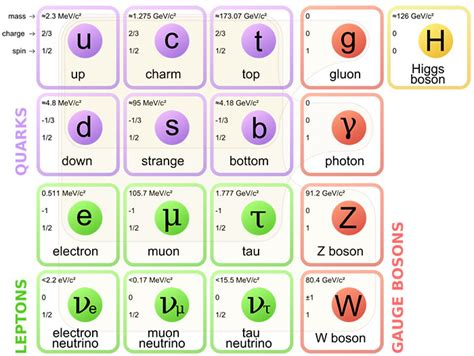
\includegraphics[width=0.5\textwidth]{standard_model.png}
When looking outside into the night sky you might see various stars, but invisible to the naked eye
various kinds of particles are also transversing light-years to end up where you stand.

When looking at phenomena outside our earth the astronomer will turn to electromagnetic radiation, as
a lot of the most interesting events emit photons in some kind of way this is very useful but he's missing
out on a big part of the full picture. That's where the astroparticle physicist comes in who takes a 
look at muons, nuclei,... and even neutrinos.

Neutrinos are ideal messengers to identify sources of ultra high energy (UHE) cosmic rays in the universe.
They also interact very weakly making it possible for them to traverse large distances unhindered. 
To fully grasp how little they interact consider that
on average 100 trillion neutrinos pass through your body per second, none of them having any effect.
You'd also need a light year of lead to give you a 50\% chance of stopping a neutrino.
\section{Discovery}
When researching beta decay, the decay of a neutron, researcher
detected a proton and an electron coming from the neutron. However
on closer inspection it became apparent that energy was lost
somewhere in violation with the conservation law of energy, and
angular momentum wasn't conserved.  The solution postulated by
Wolfgang Pauli was to introduce a new, really hard to detect
particle: the neutrino.  The neutrino comes in three flavours:
electron, muon and tau neutrinos, each corresponding to their respective lepton 
and each also having an anti-particle.
Now with the introduction of the neutrino the full beta decay
becomes
\begin{equation}
	n \rightarrow p^+ + e^- + \nu_e
\end{equation}
The inverse can then also be used to detect neutrinos:
\begin{equation}
	n \rightarrow p^+ + e^- + \nu_e
\end{equation}
Which is called beta capture and was first experimentally detected in 1956 \cite{BetaCapture} also 
making it the first experimental detection of a neutrino
\section{Neutrino sources}

\section{Do neutrinos have mass?}
Neutrinos get produced through the following ways in the nucleus of our star:\\
$\bold{pp-cycle}$
\begin{align}
	\mathrm{p} + \mathrm{p} &\rightarrow \mathrm{D} + e^+ + \nu_e\\
	\mathrm{D} + \mathrm{p} &\rightarrow {}^3\mathrm{He} + \gamma\\
	{}^3\mathrm{He} + {}^3\mathrm{He} &\rightarrow {}^4\mathrm{He} + \mathrm{p} + \mathrm{p}
\end{align}\\
$\bold{boron-cycle}$
\begin{align}
{ }^4 \mathrm{He}+{ }^3 \mathrm{He} & \rightarrow{ }^7 \mathrm{Be}+\gamma \\
{ }^7 \mathrm{Be}+p & \rightarrow { }^8\mathrm{B} + \gamma \\
{ }^8 \mathrm{B} & \rightarrow{ }^8 \mathrm{Be}^*+e^{+}+\nu_e \\
{ }^8 \mathrm{Be}^* & \rightarrow{ }^4 \mathrm{He}+{ }^4 \mathrm{He}
\end{align}\\
$\bold{Be-capture}$
\begin{align}
	^7\mathrm{Be} + e^- \rightarrow {}^7\mathrm{Li} + \nu_e
\end{align}
$\bold{pep}$
\begin{align}
	\mathrm{p} + e^- + \mathrm{p} \rightarrow \mathrm{D} + \nu_e
\end{align}\\
Now with this and some information about the sun like the pressure and mass, 
the so-called "standard solar model" was
made. This model predicted a certain amount of neutrinos to be hitting the earth from the previously
mentioned thermonuclear fusion, it was however 3 times higher than the observed amount of neutrinos back
at our planet. Through various experiments it became apparent that this was due to the various kind of
neutrinos oscillating into each other, i.e 2/3 of the original electron 
neutrinos had oscillated into mu and tau neutrinos
but for them to oscillate into eachother, they require mass:
\subsection{neutrino oscillations}
So the transition probability is
\begin{equation}
	P(\nu_e\rightarrow\nu_\mu) = |\braket{\nu_\mu|\psi(L,T)}|^2 = c_\mu c_\mu^* = \sin ^2(2 \theta) \sin ^2\left(\frac{\Delta \phi_{12}}{2}\right)
\end{equation}
with
\begin{equation}
	\Delta \phi_{12} \approx \frac{m_1^2 - m_2^2}{2p}L
\end{equation}
I.e not only mass but difference in mass of the eigenstates is a requirement for oscillations to occur.
In general
\begin{equation}
	\ket{\nu_\alpha} = \sum_iU_{\alpha i} \ket{\nu_i}
\end{equation}
With $U_{\alpha i}$ e.g the Pontecorvo-Maki-Nakagawa-Sakata (PMNS) matrix. 
This phenomenon has been observed e.g from the descrepency from the observed
and expected neutrino events coming from a nuclear reactor \cite{Eguchi_2003}.
Now the question remains, how do neutrinos get their mass (theoretically)?
\subsection{See-saw mechanism}
We can give neutrino's mass as with any other spinor throught Yukawa couplings and an extra term:
\begin{equation}
	\mathcal{L} = i\bar{\nu}\slashed{\partial}\nu - m\bar{\psi}\nu - \frac{M}{2} (\bar{\nu}_R\nu_{Rc} + \bar{\nu}_{Rc}\nu_R)
\end{equation}
More general, given a spinor $\psi$ with the following Lagrange density:
\begin{equation}
	\mathcal{L} = i\bar{\psi}\slashed{\partial}\psi - m\bar{\psi}\psi - \frac{M}{2} (\bar{\psi}_R\psi_{Rc} + \bar{\psi}_{Rc}\psi_R)
\end{equation}
We can re-write this Lagrangian in terms of
\begin{align}
	\chi &:= \frac{1}{\sqrt{2}} (\psi_R + \psi_{Rc})\\
	\omega &:= \frac{1}{\sqrt{2}} (\psi_L + \psi_{Lc})
\end{align}
by first identifying that
\begin{equation}
	- \frac{M}{2} (\bar{\psi}_R\psi_{Rc} + \bar{\psi}_{Rc}\psi_R)
\end{equation}
is equal to
\begin{equation}
	-M\bar{\chi} \chi = -\frac{M}{2} (\bar{\psi}_R + \bar{\psi}_{Rc}) (\psi_R + \psi_{Rc}) = -\frac{M}{2} (\bar{\psi}_R\psi_{Rc} + \bar{\psi}_{Rc}\psi_R)
\end{equation}
Where we've used
\begin{equation}
	\bar{\psi}_R\psi_{R} \equiv \psi_R^\dagger\gamma^0\psi_{R} \equiv P_R\psi^\dagger\gamma^0P_R\psi = P_RP_L\psi^\dagger\gamma^0\psi = 0
\end{equation}
And next that in
\begin{equation}
	i\bar{\psi}\slashed{\partial}\psi - m\bar{\psi}\psi = i\bar{\psi}_R\slashed{\partial}\psi_{R} + i\bar{\psi}_L\slashed{\partial}\psi_{L} - m\bar{\psi}_R\psi_{L} - m\bar{\psi}_L\psi_{R}
\end{equation}
We can identify that
\begin{align}
	\bar{\chi}\slashed{\partial}\chi &= \frac{1}{2}(\bar{\psi}_R\slashed{\partial}\psi_{R} + \bar{\psi}_{Rc}\slashed{\partial}\psi_{Rc}) = \bar{\psi}_R \slashed{\partial} \psi_{R}\\
	\bar{\omega}\slashed{\partial}\omega &= \bar{\psi}_L \slashed{\partial} \psi_{L}
\end{align}
Where we've done an integration by parts and used $\bar{\psi}_c\gamma_\mu\chi_c = -\bar{\chi}\gamma_\mu\psi$. We thus get:
\begin{equation}
	\mathcal{L} = i\bar{\chi}\slashed{\partial}\chi +i\bar{\omega}\slashed{\partial}\omega - m\bar{\psi}_R\psi_{L} - m\bar{\psi}_L\psi_{R} -M\bar{\chi} \chi 
\end{equation}
And finally we notice that
\begin{align}
	\bar{\chi}\omega &= \frac{1}{2} \left(\bar{\psi}_R\psi_L + \bar{\psi}_R\psi_{Lc} + \bar{\psi}_{Rc}\psi_{L} + \bar{\psi}_{Rc}\psi_{Lc}\right)\\
	&=  \frac{1}{2} \left(\bar{\psi}_R\psi_L + \bar{\psi}_R\psi_{Lc} + \bar{\psi}_{Rc}\psi_{L} + \bar{\psi}_{L}\psi_{R}\right)\\
	\bar{\omega}\chi &= \frac{1}{2} \left(\bar{\psi}_L \psi_{R} + \bar{\psi}_{Lc}\psi_{R} + \bar{\psi}_L\psi_{Rc} + \bar{\psi}_{Lc}\psi_{Rc}\right)\\
	&= \frac{1}{2} \left(\bar{\psi}_L \psi_{R} + \bar{\psi}_{Lc}\psi_{R} + \bar{\psi}_L\psi_{Rc} + \bar{\psi}_{R}\psi_{L}\right)
\end{align}
As $\bar{\psi}_c\chi_c = \bar{\chi}\psi$. Summing these, we get:
\begin{align}
	\bar{\chi}\omega + \bar{\omega}\chi &= \bar{\psi}_L \psi_R + \bar{\psi}_R \psi_{L}\\
	&\quad + \frac{1}{2}\left(\bar{\psi}_R\psi_{Lc} + \bar{\psi}_{Rc} \psi_{L} + \bar{\psi}_{Lc}\psi_R + \bar{\psi}_L\psi_{Rc}\right)\\
	&= \bar{\psi}_L \psi_R + \bar{\psi}_R \psi_{L}
\end{align}
Where we've used the handedness flips a charge conjugation entails, at last we now have:
\begin{equation}
	\mathcal{L} = i\bar{\chi}\slashed{\partial}\chi +i\bar{\omega}\slashed{\partial}\omega - m(\bar{\chi}\omega + \bar{\omega}\chi) -M\bar{\chi} \chi 
\end{equation}
Now to determine the mass eigenstates we'll re-write this equation into the form
\begin{equation}
	\mathcal{L} = i\bar{\chi}\slashed{\partial}\chi +i\bar{\omega}\slashed{\partial}\omega 
	-\left(\begin{array}{cc}
		\bar{\chi} &\bar{\omega}
	\end{array}\right)\cdot
	\left(\begin{array}{cc}
		M & m \\
		m & 0
	\end{array}\right) \cdot \left(\begin{array}{c}
	\chi \\ \omega
\end{array}\right)
\end{equation}
lets now find the eigenvalues:
\begin{equation}
	\left| \begin{array}{cc}
		M-\lambda & m \\
		m & -\lambda
	\end{array} \right| = (\lambda-M)\lambda - m^2 = 0 \implies \lambda_\pm  = \frac{M\pm \sqrt{M^2 + 4m^2}}{2} \label{eigenvalues}
\end{equation}
i.e
\begin{equation}
	\lambda_\pm = \frac{M}{2}\left( 1 \pm \sqrt{1 + 4m^2/M^2}\right)
\end{equation}
Now we'll determine the eigenvectors:
\begin{equation}
\left[\begin{array}{cc}
	M-\lambda_\pm & m \\
	m & -\lambda_\pm
\end{array}\right] \left(\begin{array}{c}
x_\pm \\
y_\pm
\end{array}\right) = \vec{0}
\end{equation}
this gives
\begin{align}
	Mx_\pm - \lambda_\pm x_\pm + my_\pm &= 0\\
	m x_\pm - \lambda_\pm y_\pm &= 0 \implies \frac{m x_\pm}{\lambda_\pm} = y_\pm
\end{align}
inserting the second equation in the first we get:
\begin{align}
	Mx_\pm - \lambda_\pm x_\pm + m \frac{m x_\pm}{\lambda_\pm} = 0 &= M\lambda_\pm x_\pm - \lambda_\pm^2 x_\pm + m^2 x_\pm\\
	&= x_\pm(\lambda_\pm^2 -M\lambda_\pm + m^2)
\end{align}
which is true for every $x_\pm$ (see equation \ref{eigenvalues}) i.e we can freely choose $x_\pm$ so let's opt for $x_\pm^2 + y_\pm^2 = 1$:
\begin{align}
	x_\pm^2(1+\frac{m^2}{\lambda_\pm^2}) = 1 \implies x^2_\pm = \frac{1}{1+\frac{m^2}{\lambda_\pm^2}} \implies x_\pm &= \frac{\lambda_\pm}{\sqrt{\lambda_\pm^2 + m^2}}\\
	\& \quad y_\pm &= \frac{m}{\sqrt{\lambda_\pm^2 + m^2}}
\end{align}
And thus, summing up, we get the eigenvectors $\phi_\pm$ with eigenvalues $m_\pm$:
\begin{equation}
	\phi_\pm := \left(\begin{array}{c}
		x_\pm\\
		y_\pm
	\end{array}\right) = \left(\begin{array}{c}
		\frac{\lambda_\pm}{\sqrt{\lambda_\pm^2 + m^2}}\\
		\frac{m}{\sqrt{\lambda_\pm^2 + m^2}}
	\end{array}\right) \quad \text{ and }\quad m_\pm := \lambda_\pm =  \frac{M}{2}\left( 1 \pm \sqrt{1 + 4m^2/M^2}\right)
\end{equation}
Now we'll consider the limit $M \gg m$:
\begin{equation}
	m_\pm =  \frac{M}{2}\left( 1 \pm \sqrt{1 + 4m^2/M^2}\right) \approx \frac{M}{2}\left(1\pm1\pm\frac{2m^2}{M^2}\right)
\end{equation}
Which gives:
\begin{align}
	m_+ &\approx M\\
	m_- &\approx -\frac{m^2}{M}
\end{align}
and:
\begin{align}
	\phi_+&\approx \left(\begin{array}{c}
		\frac{M}{M}\\
		\frac{m}{M}
	\end{array}\right) = \left(\begin{array}{c}
	1\\
	m/M
	\end{array}\right)\\
	\phi_-&\approx \left(\begin{array}{c}
		-\frac{m}{M}\\
		\frac{m}{m}
	\end{array}\right) = \left(\begin{array}{c}
		-m/M\\
		1
	\end{array}\right)
\end{align}
i.e, in the $\chi,\omega$ basis:
\begin{align}
	m_+\approx M \quad &\text{with eigenstate} \quad \chi + \frac{m}{M}\omega\\
	m_-\approx -\frac{m^2}{M} \quad &\text{with eigenstate} \quad  \omega - \frac{m}{M}\chi\\
\end{align}
This is what's called the See-Saw mechanism, it's both a theory of giving mass to
neutrinos and explaining their small mass.  
For a certain $m$ if we choose a big $M$ we'll
get a big $m_+$ and small $m_-$ (and vice versa). We also see that there's only
a very small mixing of states, i.e the $m_-$ mass state is almost purely
$\omega$ (and $m_+$ almost purely $\chi$). The parameter $m$ in the original
matrix is forbidden by electroweak gauge symmetry, and can only appear after
the symmetry has been spontaneous broken by a Higgs mechanism; for this reason
a good estimate of the order of $m$ is the vaccuum expectation energy:
$m\approx v = 246 \approx 10^2$GeV. In grand unified theories it's theorised
that $M\approx 10^{15}$GeV after symmetry breaking, using these values we get
\begin{align}
	m_- \approx 10^{-11}\text{GeV} \approx 10^{-2} \text{eV}
\end{align}
which seems \cite{neutrino-mass} to be a reasonable order of magnitude estimate for the observed neutrino
mass.
This mechanism would also lead to supermassive neutrinos, which are a possible dark matter
candidate.
\subsection{Majorana fermions}
A theory that's also quite interesting is that
neutrinos are majorana,
a dirac fermion has the following density:
\begin{align}
  \mathcal{L} &= i\bar{\psi}\slashed{\partial}\psi - m\bar{\psi}\psi\\
              &= i\bar{\psi}_L\slashed{\partial}\psi_L + i\bar{\psi}_R\slashed{\partial}\psi_R - m\bar{\psi}_R\psi_L - m\bar{\psi}_L\psi_R
\end{align}
Now assume that we only have right-handed particles:
\begin{equation}
  \mathcal{L} = i\bar{\psi}_R\slashed{\partial}\psi_R - \frac{M}{2}\bar{\psi}_R\psi_{Rc} - \frac{M}{2}\bar{\psi}_{Rc}\psi_R
\label{eqn:right-handed}
\end{equation}
A majorana fermion is a fermion which is it's own anti-particle, i.e:
\begin{align}
  \chi = \frac{1}{\sqrt{2}}\left( \psi_R + \psi_{Rc}  \right) = \chi_c
\end{align}
With this we have that
\begin{equation}
  \bar{\chi}\chi = \frac{1}{2}\left(\bar{\psi}_R\psi_{Rc} + \bar{\psi}_{Rc}\psi_R\right)
\end{equation}
Which we can recognize in \ref{eqn:right-handed} and
\begin{align}
  \bar{\chi}\slashed{\partial}\chi &= \frac{1}{2}(\bar{\psi}_R + \bar{\psi}_{Rc}) \slashed{\partial}(\psi_R + \psi_{Rc})\\
                                   &= \frac{1}{2} \bar{\psi}_R\slashed{\partial}\psi_R + \frac{1}{2}\bar{\psi}_{Rc}\slashed{\partial}\psi_{Rc}\\
                                   &= \bar{\psi}_R \slashed{\partial}\psi_R
\end{align}
where we've used integration by parts at the end, with these we can re-write \ref{eqn:right-handed} as:
\begin{equation}
  \mathcal{L} = i\bar{\chi}\slashed{\partial}\chi - M \bar{\chi}\chi
\end{equation}
Thus arriving at a density for Majorana fermions with mass M, a possible detection mechanism
to find out if neutrinos are Majorana is "Neutrinoless double beta decay":
\begin{figure}[h!]
	\begin{minipage}{\textwidth}
		\begin{minipage}{0.49\textwidth}
			\centering
			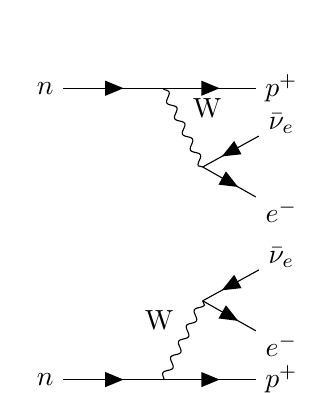
\begin{tikzpicture}
				\begin{feynman}
					\vertex (a0) {\(n\)};
					\vertex[right=3cm of a0] (a1) {\(p^+\)};
					\vertex[right=1.5cm of a0] (am);
					\vertex[right=0.5cm of am] (awi);
					\vertex[above=1cm of awi] (aw);
					\vertex[right=1cm of aw] (avm);
					\vertex[above=0.3cm of avm] (av1) {\(\bar{\nu}_e\)};
					\vertex[below=0.3cm of avm] (av0) {\(e^-\)};
					
					\vertex[above=3.7cm of a0] (b0) {\(n\)};
					\vertex[right=3cm of b0] (b1) {\(p^+\)};
					\vertex[right=1.5cm of b0] (bm);
					\vertex[right=0.5cm of bm] (bwi);
					\vertex[below=1cm of bwi] (bw);
					\vertex[right=1cm of bw] (bvm);
					\vertex[above=0.3cm of bvm] (bv1) {\(\bar{\nu}_e\)};
					\vertex[below=0.3cm of bvm] (bv0) {\(e^-\)};
					
					\diagram* {
						{[edges=fermion]
							(a0) -- (am) -- (a1)
						},
						{[edges=boson,edge label= W]
							(am) -- (aw)
						},
						{(av1) -- [fermion] (aw) --[fermion] (av0)},
						
						{[edges=fermion]
							(b0) -- (bm) -- (b1)
						},
						{[edges=boson,edge label= W]
							(bm) -- (bw)
						},
						(bv1) -- [fermion] (bw) --[fermion] (bv0),
						
					};
				\end{feynman}
			\end{tikzpicture}
		\end{minipage}
		\begin{minipage}{0.49\textwidth}
			\centering
			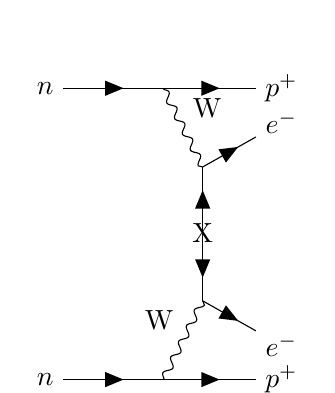
\begin{tikzpicture}
				\begin{feynman}
					\vertex (a0) {\(n\)};
					\vertex[right=3cm of a0] (a1) {\(p^+\)};
					\vertex[right=1.5cm of a0] (am);
					\vertex[right=0.5cm of am] (awi);
					\vertex[above=1cm of awi] (aw);
					\vertex[right=1cm of aw] (avm);
					\vertex[above=0.85cm of aw] (av1);
					\vertex[below=0.3cm of avm] (av0) {\(e^-\)};
					
					\vertex[above=3.7cm of a0] (b0) {\(n\)};
					\vertex[right=3cm of b0] (b1) {\(p^+\)};
					\vertex[right=1.5cm of b0] (bm);
					\vertex[right=0.5cm of bm] (bwi);
					\vertex[below=1cm of bwi] (bw);
					\vertex[right=1cm of bw] (bvm);
					\vertex[below=0.85cm of bw] (bv1);
					\vertex[above=0.3cm of bvm] (bv0) {\(e^-\)};
					\vertex[below=0.6cm of bw] (ann) {X};
					
					\diagram* {
						{[edges=fermion]
							(a0) -- (am) -- (a1)
						},
						{[edges=boson,edge label= W]
							(am) -- (aw)
						},
						{(av1) -- [fermion] (aw) --[fermion] (av0)},
						
						{[edges=fermion]
							(b0) -- (bm) -- (b1)
						},
						{[edges=boson,edge label= W]
							(bm) -- (bw)
						},
						(bv1) -- [fermion] (bw) --[fermion] (bv0),
						
					};
				\end{feynman}
			\end{tikzpicture}
		\end{minipage}
	\end{minipage}
	\caption{normal and neutrinoless double beta decay}
\end{figure}\\
This is (at the time of writing) actively investigated.
\section{Why study neutrinos?}
%The radio detection of neutrinos targets the energy range 10PeV to 100EeV\cite{Aguilar_2021} 
Neutrinos are ideal messengers to identify the UHE (Ultra High Energy) sources
in the universe. Unlike cosmic rays, which are deflected by magnetic fields and
interact with matter and radiation on their way to us, neutrinos point back to
sources and can reach Earth unperturbed from the most distant corners of the
universe.  Neutrinos can be generated in 2 ways: either they're generated in
interactions at the sources, termed \textit{astrophysical neutrinos}. Or
they're created through the interaction of ultra-high energy cosmic rays during
propagation with the cosmic microwave or other photon backgrounds termed
\textit{cosmogenic neutrinos}. 
\subsection{astrophysical neutrinos: general}
As cosmic rays get accelerated they will occasionally interact with matter
and photon fields near the source. These will then produce new particles,
of which the most common is pions due to their low mass (a lot of available 
phase space). As seen in chapter \ref{chapter:EWTheory} pions can decay
into neutrino's as follows:
\begin{eqnarray}
	\pi^- &\rightarrow \mu^- + \bar{\nu}_\mu \rightarrow e^- + \bar{\nu}_e + \nu_\mu + \bar{\nu}_\mu\\
	\pi^+ &\rightarrow \mu^+ + \nu_\mu \rightarrow e^+ + \nu_e + \bar{\nu}_\mu + \nu_\mu
\end{eqnarray}
Another possibility is direct production of neutrino's at the source, of which Supernovae are
a prime example:
\subsection{Supernovae}
A star starts its life as a ball of pure hydrogen. At the core, due to the
gravitational pressure of the outside plasma, fusion of hydrogen into deuterium
and helium happens. Thus converting mass into energy. The pressure of this energy
counteracts the pressure of gravity and the star is stable.

When the hydrogen at the core runs out no more hydrogen can be fused. For
stars with masses between $8M_\odot$ and $30M_\odot$ the
fusion of heavier elements starts, this can't keep going on however as at some
point the star starts to form the most stable element: iron. 
\begin{figure}[!ht]
	\centering
	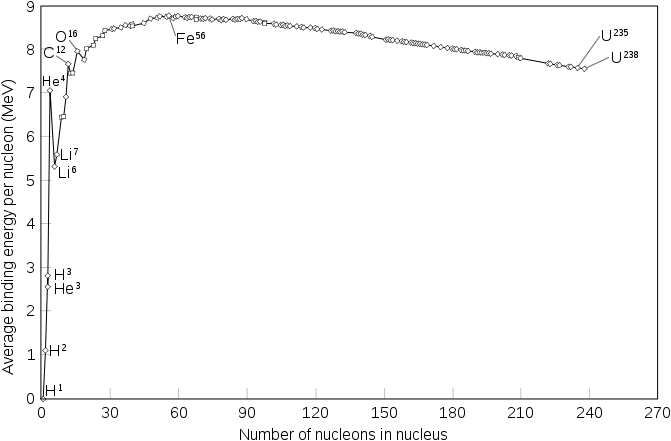
\includegraphics[width=0.5\textwidth]{Binding_energy_curve.png}
\end{figure}
It costs energy
to both make lighter elements than iron and heavier ones.  As the iron core
builds up the outside pressure from the core starts to decrease as no new
energy is released. This goes on until  the treshold of an iron core with a mass of 1.4$M_\odot$ known as the 
Chandrasekhar limit and the the inwards pressure becomes too large, making the electrons surrounding the 
iron core fuse with the protons (uud),  creating neutrons (udd) and neutrino's, diagramatically:
\begin{figure}[!ht]
	\centering
	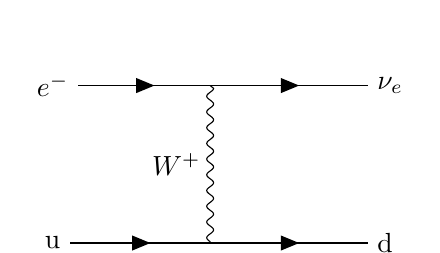
\begin{tikzpicture}
	\begin{feynman}
	\vertex (a0){u};
	\vertex[right=2cm of a0] (am) ;
	\vertex[right=2cm of am] (a1) {d};
	\vertex[above=2cm of am] (bm);
	\vertex[above=2cm of a0] (b0){$e^-$};
	\vertex[right=2cm of bm] (b1){$\nu_e$};
	\diagram* {
		{[edges=fermion]
			(a0) -- (am) -- (a1)
		},
		{[edges=fermion]
			(b0) -- (bm) -- (b1)
		},
		{[edges=boson,edge label=$W^+$]
			(am) -- (bm)
		}
	};
	\end{feynman}
	\end{tikzpicture}
\end{figure}\\
This last part happens in a split second as the collapse goes at 25\% the speed of light, 
creating a very dense neutron star (3000km in diameter iron core to 30km in diameter neutron star) 
and up to $10^{52}$ ultra-relativistic neutrinos, carrying up to 99\% of the
released energy \cite{Melson_2015}\footnote{1\% is released as kinetic energy, only 0.001\% as electromagnetic radiation}.
As the density has suddenly
increased so much there's a huge distance of pure vaccuum between the plasma
outer layer and the (now) neutron star, this plasma starts free-falling inwards, 
also at 25\% the speed of light whilst the neutrinos carrying tremendous amounts 
of energy start going outwards from the neutron stars core.

The neutrinos then collide with the plasma resulting in what we observe as a "supernova", wrongly
thought of by Kepler as being a "new (nova) star" rather being a violent death
of an old star.

This is quite unexpected as neutrinos rarely interact, they only do becouse the
incoming plasma is so dense and due to the tremendous amount of neutrinos that 
collissions happen at all. Some, however, escape and will be visible on earth in 
our neutrino detectors $\approx$ 18h before the light escapes the exploding star.

Neutrino observatories are thus useful to know where to point our various
telescopes before the supernova is actually visible in the night sky.
\subsection{primordial neutrinos}
Aside from all the previously mentioned sources, there's also a less spectacular source of 
neutrinos: the neutrino version of the CMB.
We can estimate the temperature of the neutrinos who decoupled at the start of the universe, 
for this we can take a look at conservation of entropy \cite{Dodelson}
\begin{equation}
	T_\nu = \left(\frac{4}{11}\right)^{1/3}T_\gamma
\end{equation}
\subsection{How do they fit into the full detector spectrum?}
The origin of the most energetic cosmic rays is still not conclusively
identified. One approach to solving this problem is \textit{multi-messenger
astrophysics}, where several types of cosmic particles are used to identify the
sources of these ultra-high energy cosmic rays (UHECRs). E.g we simultaneously
measure gravitational waves (gravitons?) with the Einstein telescope,
neutrino's with IceCube (or eventually RNO-G), photons with various telescopes
and muons with a muon detector.
\newpage
\chapter{Radio detection of neutrinos}
\section{Neutrino interactions in ice}
As neutrinos propagate through ice they can interact with nuclei in the following ways\cite{NuRadioMc}:
\begin{figure}[h!]
	\begin{minipage}{\textwidth}
		\begin{minipage}{0.49\textwidth}
			\centering
			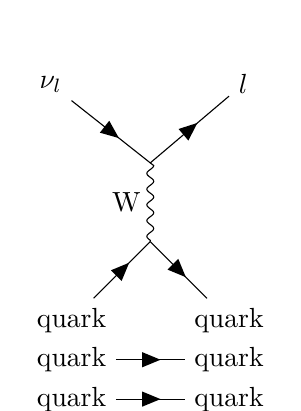
\begin{tikzpicture}
				\begin{feynman}
					\vertex (a0) {quark};
					\vertex[above=0.5cm of a0] (a1) {quark};
					\vertex[above=0.5cm of a1] (a2) {quark};
					\vertex[right=2cm of a0] (b0) {quark};
					\vertex[right=2cm of a1] (b1) {quark};
					\vertex[right=2cm of a2] (b2) {quark};
					\vertex[right=1.0cm of a2] (am);
					\vertex[above=1cm of am] (c0);
					\vertex[above=1cm of c0] (c1);
					\vertex[above=1cm of c1] (cm);
					\vertex[left=1cm of cm] (a3) {$\nu_l$};
					\vertex[right=1cm of cm] (b3) {$l$};
					\diagram* {
						{[edges=fermion]
							(a0) -- (b0)
						},
						{[edges=fermion]
							(a1) -- (b1)
						},
						{[edges=fermion]
							(a2) -- (c0) -- (b2)
						},
						{[edges=fermion]
							(a3) -- (c1) -- (b3)
						},
						{[edges=boson, edge label=W]
							(c0) -- (c1)
						},
					};
				\end{feynman}
			\end{tikzpicture}
		\end{minipage}
		\begin{minipage}{0.49\textwidth}
			\centering
			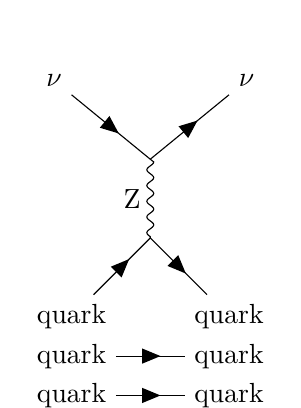
\begin{tikzpicture}
				\begin{feynman}
					\vertex (a0) {quark};
					\vertex[above=0.5cm of a0] (a1) {quark};
					\vertex[above=0.5cm of a1] (a2) {quark};
					\vertex[right=2cm of a0] (b0) {quark};
					\vertex[right=2cm of a1] (b1) {quark};
					\vertex[right=2cm of a2] (b2) {quark};
					\vertex[right=1.0cm of a2] (am);
					\vertex[above=1cm of am] (c0);
					\vertex[above=1cm of c0] (c1);
					\vertex[above=1cm of c1] (cm);
					\vertex[left=1cm of cm] (a3) {$\nu$};
					\vertex[right=1cm of cm] (b3) {$\nu$};
					\diagram* {
						{[edges=fermion]
							(a0) -- (b0)
						},
						{[edges=fermion]
							(a1) -- (b1)
						},
						{[edges=fermion]
							(a2) -- (c0) -- (b2)
						},
						{[edges=fermion]
							(a3) -- (c1) -- (b3)
						},
						{[edges=boson, edge label=Z]
							(c0) -- (c1)
						},
					};
				\end{feynman}
			\end{tikzpicture}
		\end{minipage}
	\end{minipage}
	\caption{Most prominent ways of neutrino-nucleus interaction}
\end{figure}\\
With the produced leptons in the W boson mediated interaction being either electrons,
resulting in an electromagnetic shower, muons wich typically go undetected as they live
too long or
tauons wich will decay via
\begin{equation}
	\tau^- \rightarrow e^- + \bar{\nu}_e + \nu_\tau
\end{equation}
or, less ideally
\begin{equation}
	\tau^- \rightarrow \mu^- + \bar{\nu}_\mu + \nu_\tau
\end{equation}
In both of the possible interactions the resulting nucleus will result in a 
hadronic shower, for the neutral current interaction (mediated by the Z boson) 
the fraction of the neutrino energy that gets transferred to the nucleon
is described by the inelasticity $y$ and is heavily shifted towards small
values of $y$\cite{elasticity_y}. This causes a big, irreducable uncertainty
when trying to estimate the original
neutrino energy from these kinds of events. 
With the charged current interaction (mediated by the $W^\pm$ bosons) this 
isn't a problem however as the full neutrino energy
ends up in the resulting cascades.
\section{Askaryan effect}
For a particle shower to emit strong radio signals, two conditions have to be met:
\begin{itemize}
	\item There needs to be a speration of positive and negative charges in the shower front 
	\item The signals produced over the length of the shower profile need to overlap coherently.
\end{itemize}
The \textit{Askaryan} \cite{Askaryan} effect, also known as Askaryan
radiation describes the effect at radio frequencies which abides by both 
of these conditions, in general it's a quite difficult effect but we'll give 
a crude overview. 
The above described interactions create a shower
of secondary charged particles containing a charge anisotropy, 
this charge imbalance is a result of medium electrons either Compton
scattering into the advancing shower or annihilating with shower positrons. 
In the end you have a moving charge anisotropy, propagating faster than the speed of 
light in the medium,
creating Cherenkov radiation.
Cherenkov radiation is like the elektromagnetic equivalent of a sonic boom, a
sonic boom happens when something goes faster than the sounds speed in the
medium; A particle emits Cherenkov radiation if it goes faster than the light
speed in the medium\footnote{The reader who wants a thorough explanation and derivation is
advised to check out \textit{Chapter 14: Radiation by Moving Charges} from the
book \textit{Classical Electrodynamics} by Jackson.} 
. Choosing the particle trajectory to lie along the z axis
we can approximately find an equation for $\frac{\text{d}^2 \mathscr{J}}{\text{d}\omega \text{d}\Omega}$: the energy radiated per elementary unit solid angle and per elementary unit frequency interval
\begin{equation}
	\frac{\text{d}^2 \mathscr{J}(\omega)}{\text{d} \omega \text{d} \Omega} = \frac{q^2}{4\pi}\sqrt{\frac{\mu}{\epsilon}}\beta^2\omega^2\delta^2[\omega(1-\beta \mathbf{e}_r\cdot\mathbf{e}_z)]|\mathbf{e}_r\times\mathbf{e}_z|^2 \label{equation: 4.128 in elektromagnetisme}
\end{equation}
Now we can re-write this equation in spherical coordinates, which gives $1-\beta \mathbf{e}_r\cdot\mathbf{e}_z = 1-\beta\cos(\theta_c)$ in the delta function. We thus only expect radiation if
\begin{equation}
\cos(\theta_c) = \frac{1}{\beta} = \frac{c'}{u} = \frac{c}{n}\cdot\frac{1}{u}
\end{equation}
I.e if $u>\frac{c}{n}$ with n the index of refraction, Cherenkov radiation will be emitted along a cone surface with half angle $\frac{\pi}{2}-\theta_c$ as illustrated in figure \ref{figure: Cherenkov illustratie}. Integrating equation \ref{equation: 4.128 in elektromagnetisme} over the solid angle and formally deviding by the time interval we get:
\begin{equation}
	\frac{\text{d}^2\mathscr{J}}{\text{d}\omega \text{d}t} = \frac{q^2}{4\pi}\sqrt{\frac{\mu}{\epsilon}}\beta\omega\left(1-\frac{1}{\beta^2}\right)	
\end{equation}
We see that the energy is proportional to $\omega$, so we expect that most
radiation will be emitted "in blue", as seen in figure \ref{figure: Cherenkov
reactor}.  For ice the index of refraction is roughly 1.78 in deep ice, so we
expect an ultra-relativistic particle to produce the most radiation at around
56° opening as 
\begin{equation}
	\cos(\theta_c) \approx \frac{1}{n} \implies \cos^{-1}\left(\frac{1}{1.78}\right)\approx 56\text{°}
\end{equation}
\begin{figure}
\centering
\begin{minipage}{0.45\textwidth}
	\centering
	\copyrightbox[r]{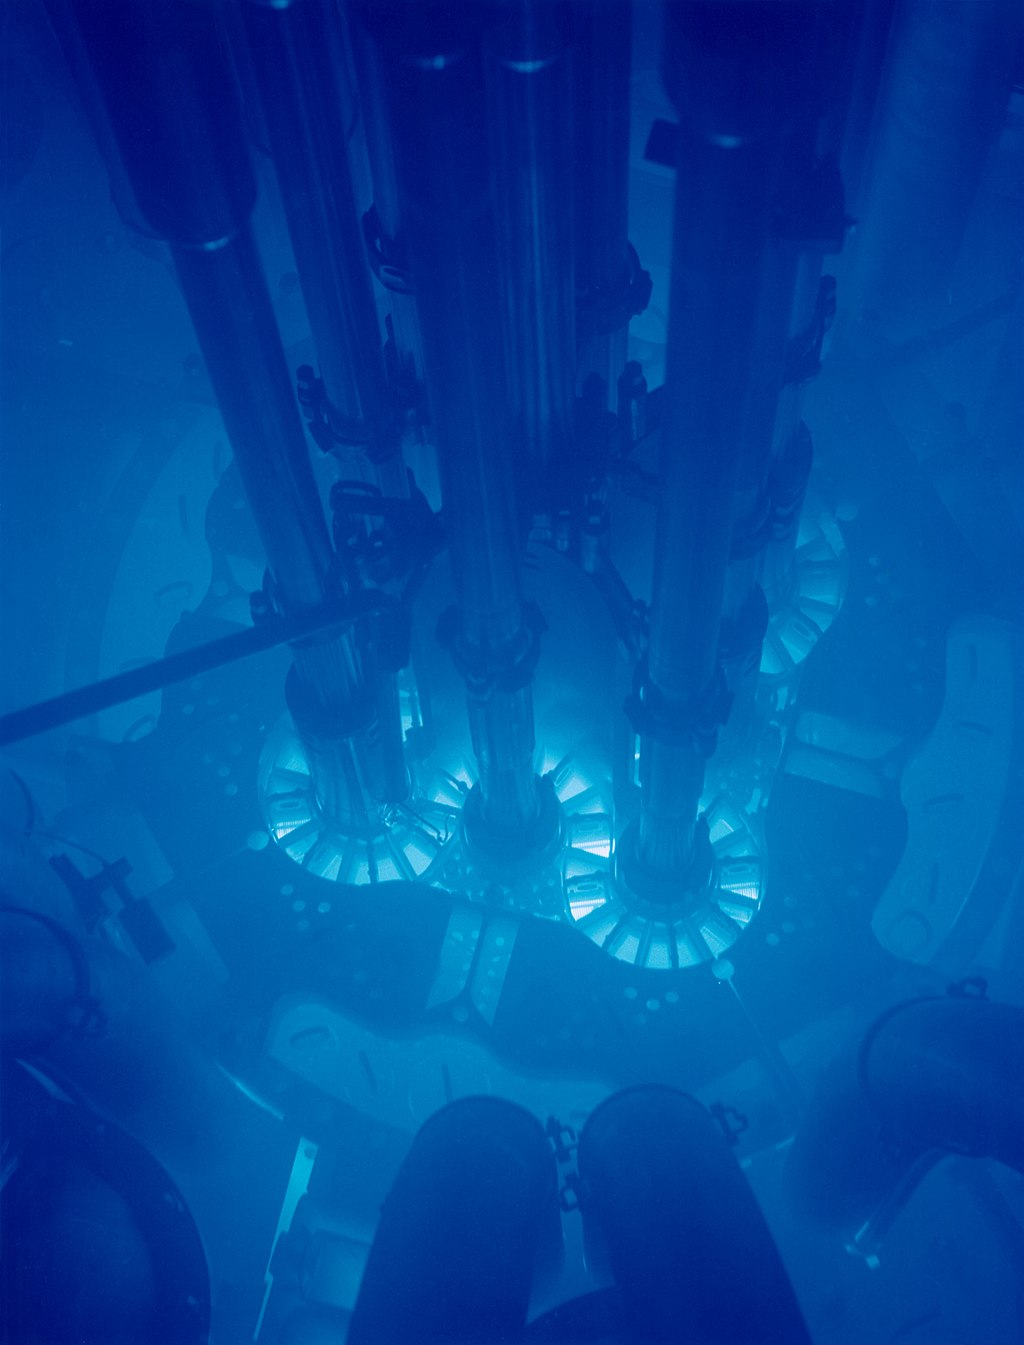
\includegraphics[height = 0.8\textwidth]{Cherenkov-reactor.jpg}}{\textcopyright Argonne National Laboratory\\Advanced Test Reactor core, Idaho National Laboratory}
	\caption{Cherenkov radiation in a nuclear reactor}
	\label{figure: Cherenkov reactor}
\end{minipage}
\hspace{0.05\textwidth}
\begin{minipage}{0.45\textwidth}
	\centering
	\copyrightbox[r]{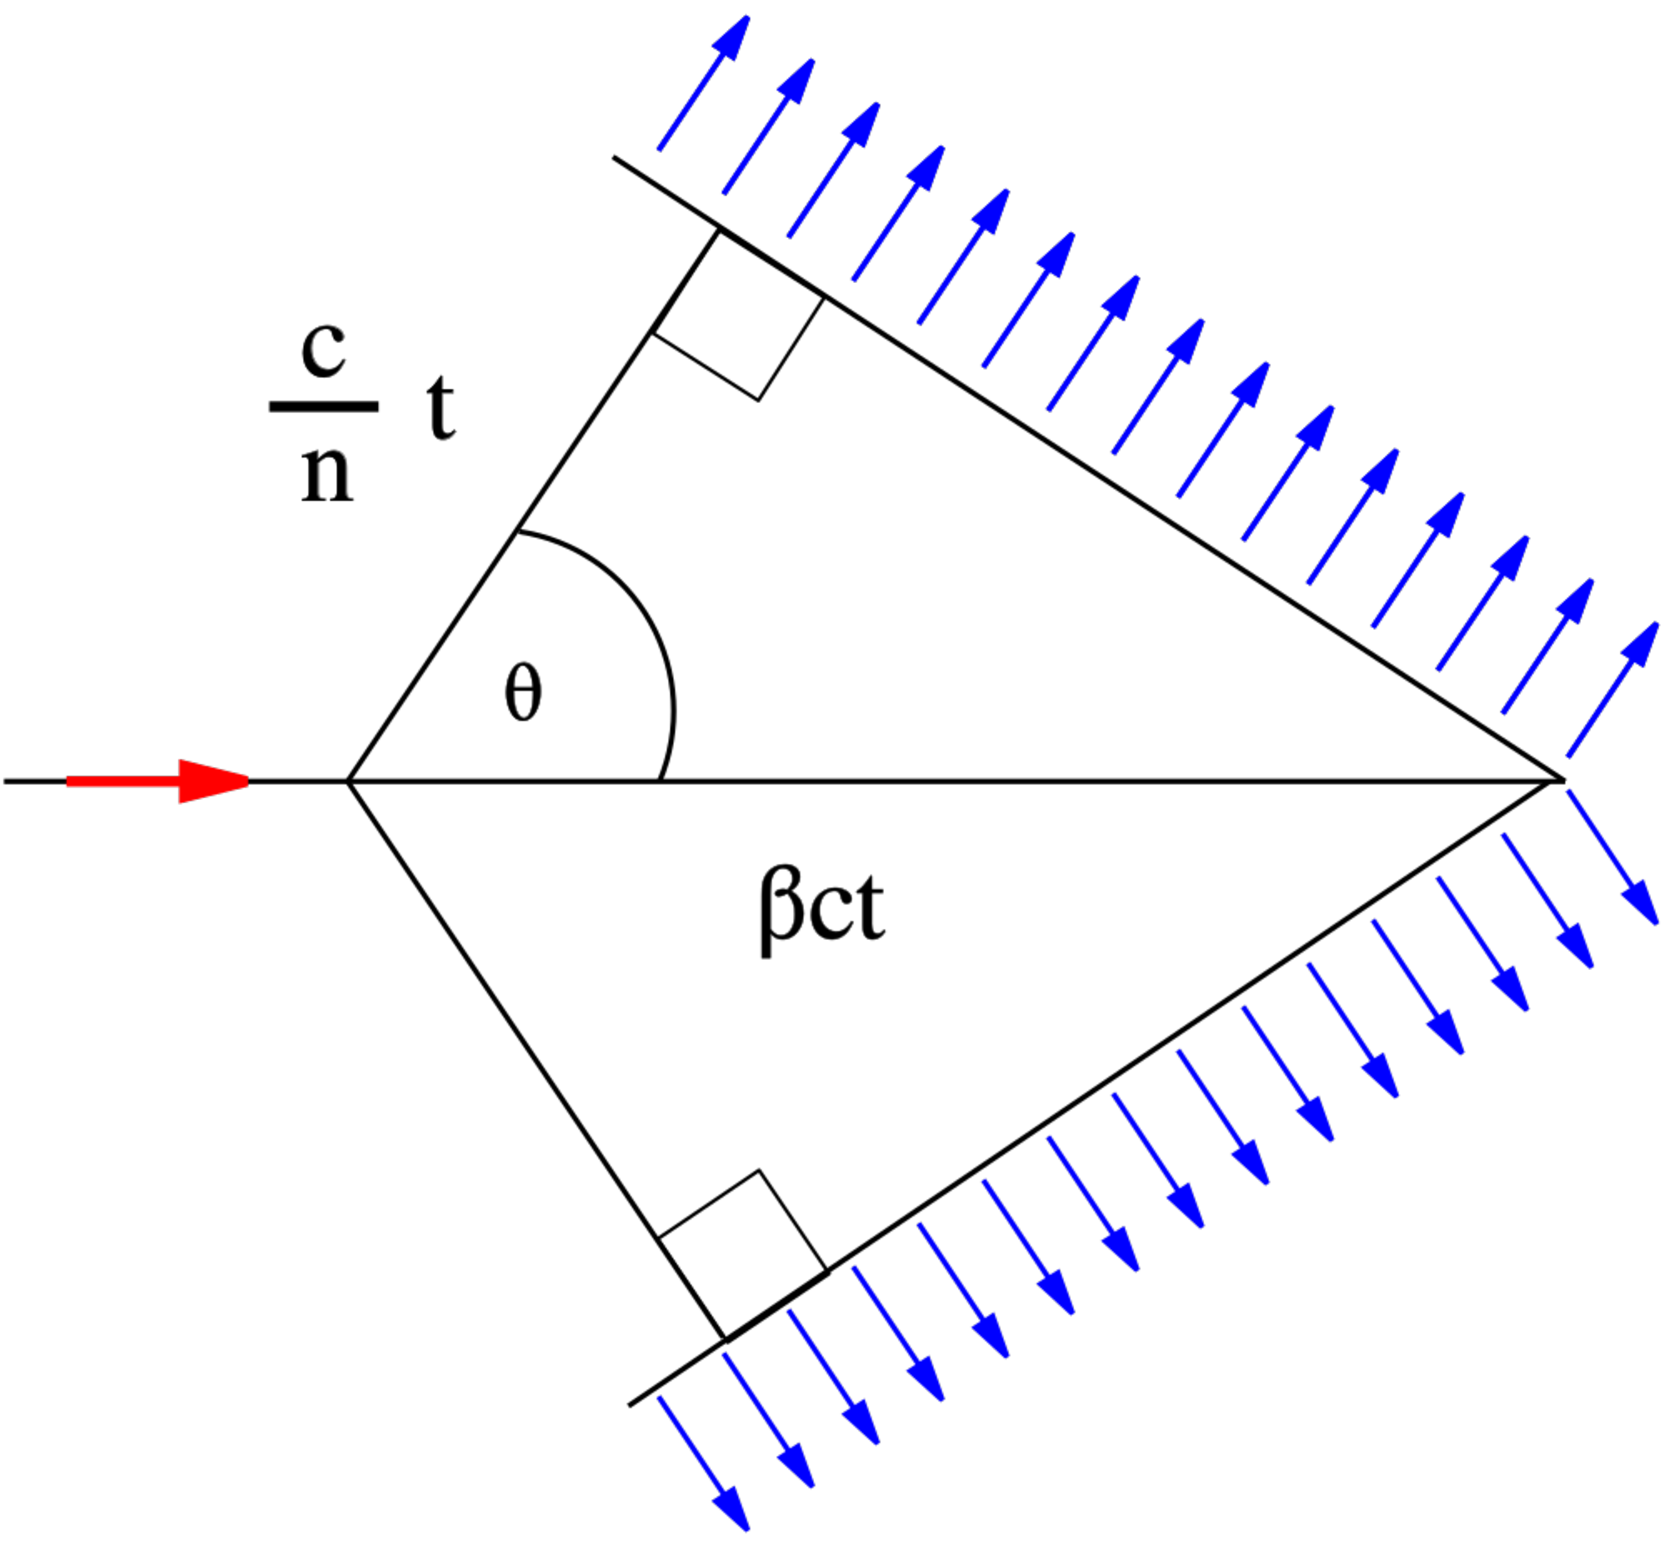
\includegraphics[height = 0.8\textwidth]{Cherenkov.pdf}}{\textcopyright Arpad Horvath}
	\caption{Diagrammatic representation of Cherenkov radiation}
	\label{figure: Cherenkov illustratie}
\end{minipage}
\end{figure}
Of course this is just an estimate, as the actual index of refraction is depth-dependent which
we'll get to in section (...).
Now this explains how the signals get generated but logically, from only knowing this
we'd expect radio waves to almost be non-existent 
due to the "in blue" nature of Cherenkov radiation. 
This isn't the full story however as we'll need to talk about coherent overlap
to fully understand the Askaryan effect. This can be intuitively explained as
follows: generally the shower is of length
$\mathcal{O}$(10cm)\cite{Huege_2017}, over this length the radiation gets
emitted, most frequencies decoherently interfering, but radio waves with wavelengths of 
$\approx$ 10cm coherently interfere, and it's these waves we then wish to detect.
\section{Wave propagation}
Waves propagating through ice to a detector generally looks something like this:
\begin{figure}[h!]
	\centering
	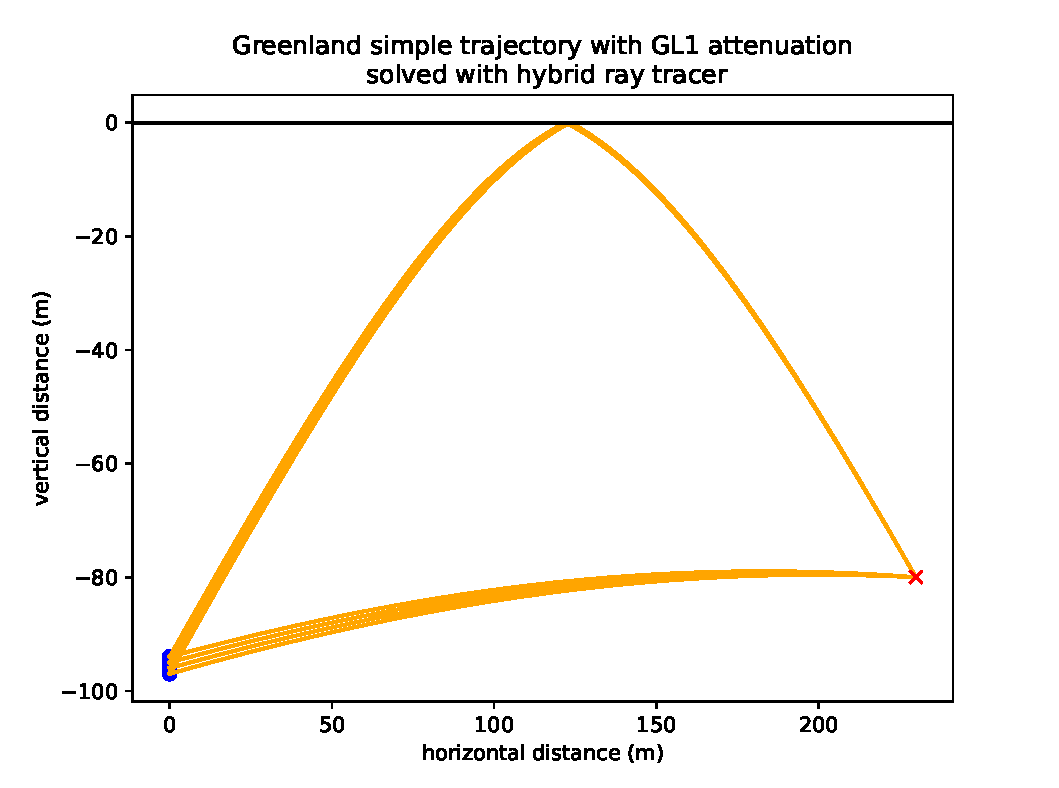
\includegraphics[width=0.7\textwidth]{Path_illu.pdf}
\end{figure}\\
Here the interaction of the neutrino happens somewhere in the neighbourhood of the red cross,
the orange rays represent the resulting radio wave paths to the detectors which are signaled
by the blue dot. Notice that reflection at the surface is also a
possible path to the detector.
In a homogeneous dielectric medium a ray propagates straight 
with it's signal wave-speed determined by the local index of 
refraction as $v = c/n$, 
the dependence of the index of refraction on density
for ice is given by the Schytt equation:
\begin{equation}
	n(x,y,z) \approx 1 + 0.78\rho(x,y,z)/\rho_0
\end{equation}
Where $\rho(x,y,z)$ is the local ice density and $\rho_0$ is the
density for solid ice (917 kg/m³).
This isn't the only part of the index of refraction with which we'll
need to concern ourselves however. If a ray propagates towards a
boundary dividing 2 media with different indexes of refraction, the
ray will refract and the refracted angle can be
found from Snell's law:
\begin{equation}
	n_1\sin{\theta_1} = n_2\sin{\theta_2}
\end{equation}
Where n is the index of refraction and $\theta$ is the angle
with respect to the surface.
The system we'll consider however, isn't 
homogeneous with some specified boundary, it's continous: ice
in greenland has a continously varying density. 
Because of this we can't work with Snell's law but we'll have to 
take a look at the continuous version
to figure out how these rays propagate. 
The "continuous version of Snell's law" is the eikonal equation:
a path of a ray $\mathbf{r}(s)$ with path parameter s in a medium
with index of refraction n($\mathbf{r}$) is described by:
\begin{equation}
	\frac{d}{ds}\left(n(\mathbf{r})\frac{d\mathbf{r}}{ds}\right) = \mathbf{\nabla} n
\end{equation}
The software we'll be using for ray reconstruction is called
"radiopropa" \cite{Winchen_2019} and in radiopropa the
local paraxial approximation is used, i.e. if we assume that in any
individual step of the algorithm the change of the refractive index
along the path ds is small it's possible to
re-write the equation as:
\begin{equation}
	n(\mathbf{r})\frac{d^2\mathbf{r}}{ds^2} \approx \mathbf{\nabla} n
	\label{eqn:radiopropaformula}
\end{equation}
Which is then easily iteratively solved.
If there are boundaries (such as defects or the surface)
these are treated seperately using Snell's law. 
\section{Ice model}
Equation \ref{eqn:radiopropaformula}, and thus the path, depends 
on the index of refraction on a given location. 
Purely from classical gravity and density considerations
it can be derived that the index of refraction abides by
\begin{equation}
	n(z) = n_{ice} - \Delta n e^{z/z_0}
\end{equation}
with $n_{ice}$ the refractive index of solid ice and $\Delta n =
n_{ice} - n_s$ with $n_s$ the index of refraction of snow. This is
called
"the exponential model".

From the measured density with depth variation this seems to
roughly hold but it could be better (as will be explained in chapter
(TBC)).
This exponential model has a huge advantage as it's analytically 
solvable, meaning that we don't have to iteratively search for the 
path to the detector but know it instantly after the location of
the neutrino interaction and the detector are specified, this
"model" is called the \textit{analytic ray tracer}.
\section{Reconstruction}
It can pose a challenge to reconstruct the radio signals produced by
the Cherenkov radiation as they are often obscured by background
noise. A solution used in RadioReco is Information Field Theory
(IFT) implemented in RadioReco by Welling et al.\cite{Welling_2021}
which uses Bayesian inference to calculate the most likely radio
signal, given recorded data.  The full reconstruction will then work
as follows: events and their propagation are generated in a
monte-carlo simulation using
NuRadioMC\cite{Glaser_2019}\cite{Glaser_2020}, how the detector
signals would look like is then simulated with RadioReco and saved
in a database.  If we then detect a neutrino event in the real
detector it can be compared to the database, thus finding the
origin.
\chapter{The Detector}
\begin{figure}
	\centering
	\copyrightbox[r]{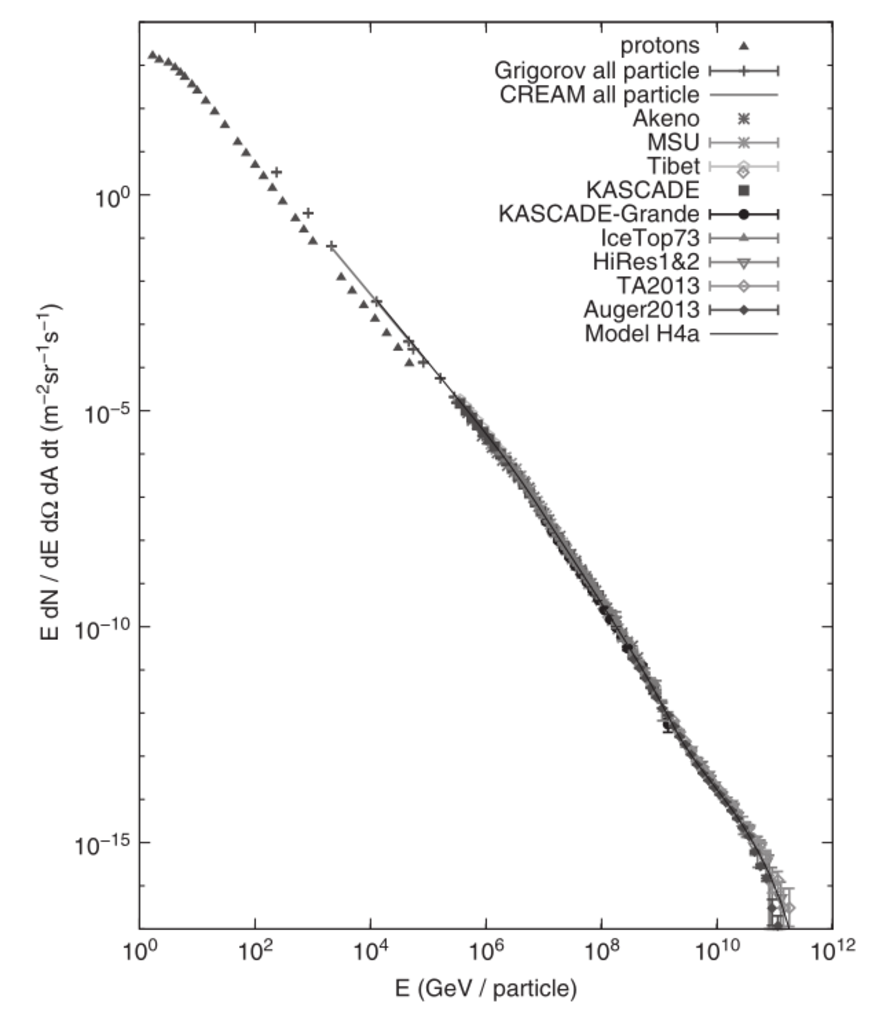
\includegraphics[height = 0.3\textheight]{cosmic_ray_flux.pdf}}{\textcopyright Cosmic rays and particle physics by Caiser, Engel and Resconi}
	\caption{Falling cosmic ray flux with energy}
	\label{figure:FallingFlux}
\end{figure}
Both cosmic ray and neutrino detectors face the same main problem at the
highest energies: the steeply falling flux (as can be seen on figure \ref{figure:FallingFlux}) 
requires large effective areas, which
leads to the construction of neutrino detectors with volumes on the cubic
kilometer scale: IceCube. As we wish to detect neutrino's with even higher
energies we turn to look at an array of detectors spanning multiple cubic
kilometers: RNO-G.

One such detector is illustrated in figure \ref{fig:detector}.

The deep component of the detector can be split up in three parts: Two \textit{helper strings}, one \textit{power string} and the surface components. The helper strings are the 2 vertical cables shown on the right of the figure and each one houses 2 vertically polarized antennas (Vpols), one quadslot antenna for the horizontal polarization component (Hpol) and one radio pulser on each helper string which can be used to generate calibration signals.

The power string (the leftmost vertical cable) is more densely instrumented: At the bottom it houses a set of four Vpol and two Hpol antennas with a spacing of 1m and further up the string, with a spacing of 20m are three more Vpol antennas.

The signal from each of these antennae are fed into a low-noise amplifier directly above it, from there the signal is send to the data acquisition (DAQ) system at the surface via a Radio Frequency over Fiber (RFoF) cable. There it's again amplified, digitized and saved onto an SD card. This data is then transmitted via a Long Term Evolution (LTE) telecommunications network to a local server\footnote{There is additionally a Long Range Wide Area Network (LoRaWAN) antenna as backup in case of problems with the LTE network}, from where it is sent via a sattelite link.

There are solar panels as a power source who charge up battery banks, but as there is't enough light during the Greenland winters, there're plans to build wind turbines (with the problem being the possibly detectable RF noise the 'engine' produces)

\begin{figure}
	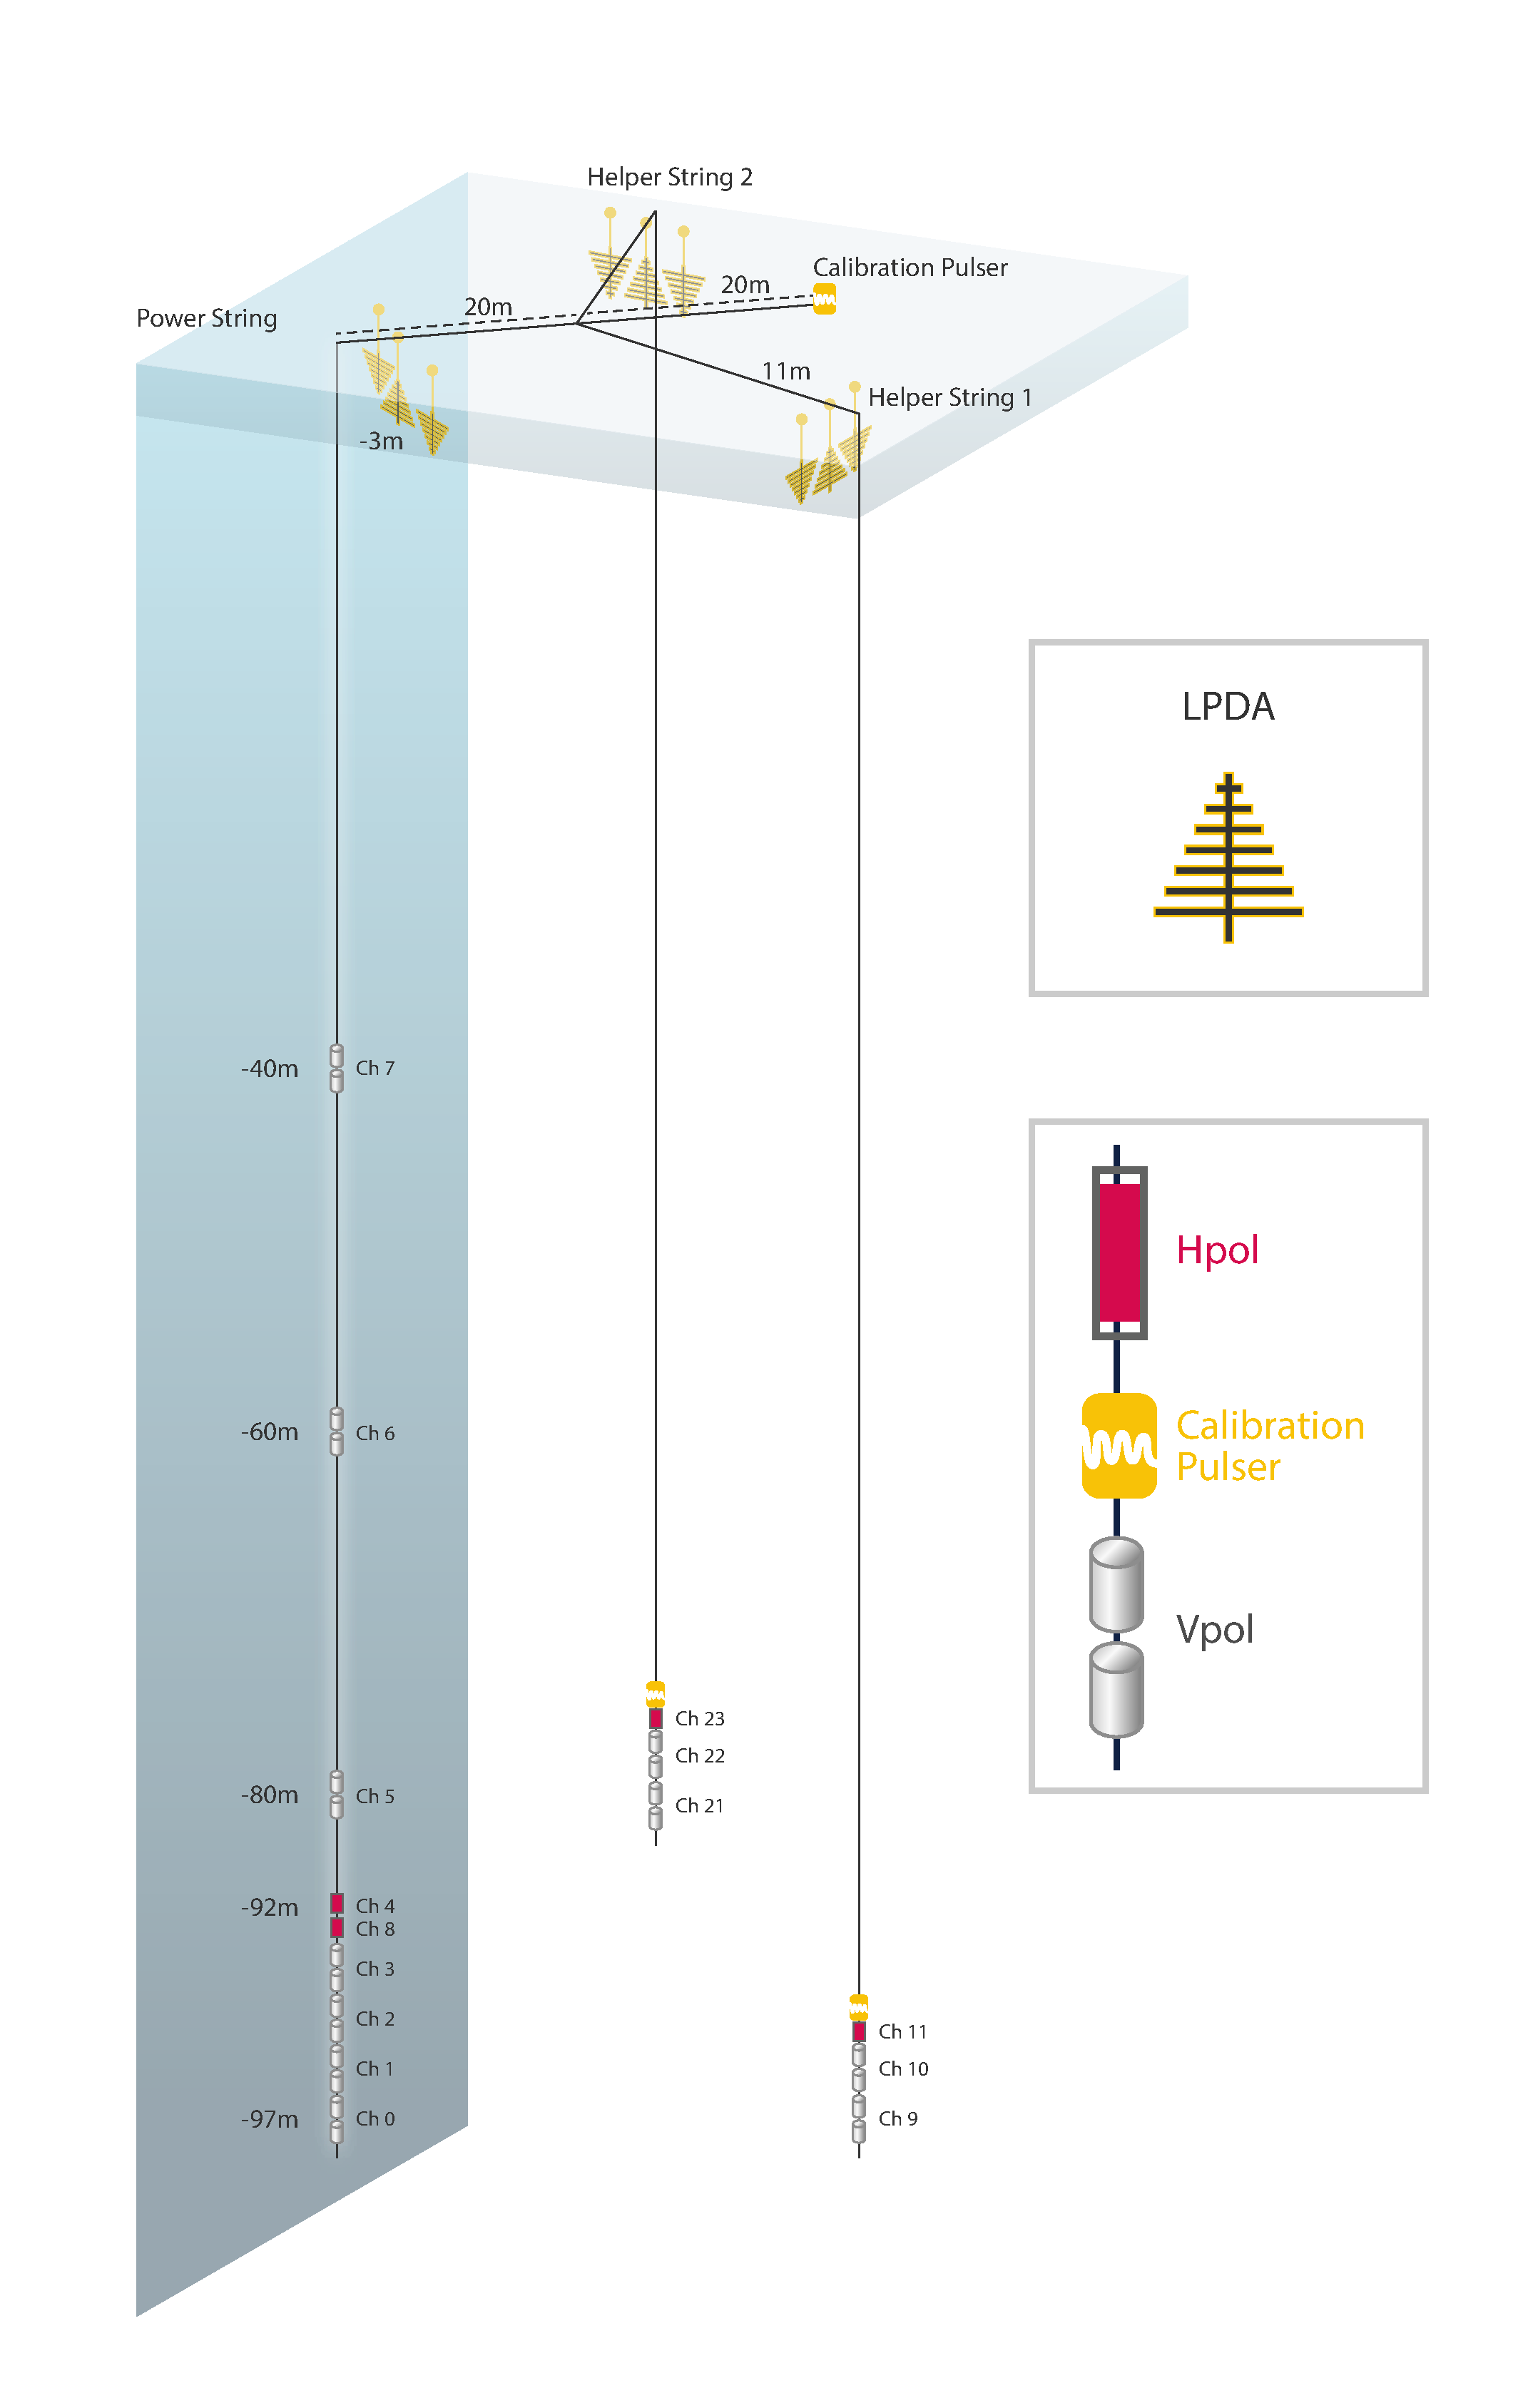
\includegraphics[width=0.9\textwidth]{figures/detector.pdf}	
	\caption{illustration of the detector}
	\label{fig:detector}
\end{figure}
\newpage
The radio signal from a neutrino often travels along both direct and refracted paths (designated DnR) to the deep array, this happens because the upper ice layer is a non-uniform medium where the signal trajectory is bent, as illustrated by a simulation in figure \ref{fig:path_illustration}. 

\begin{figure}
	\centering
	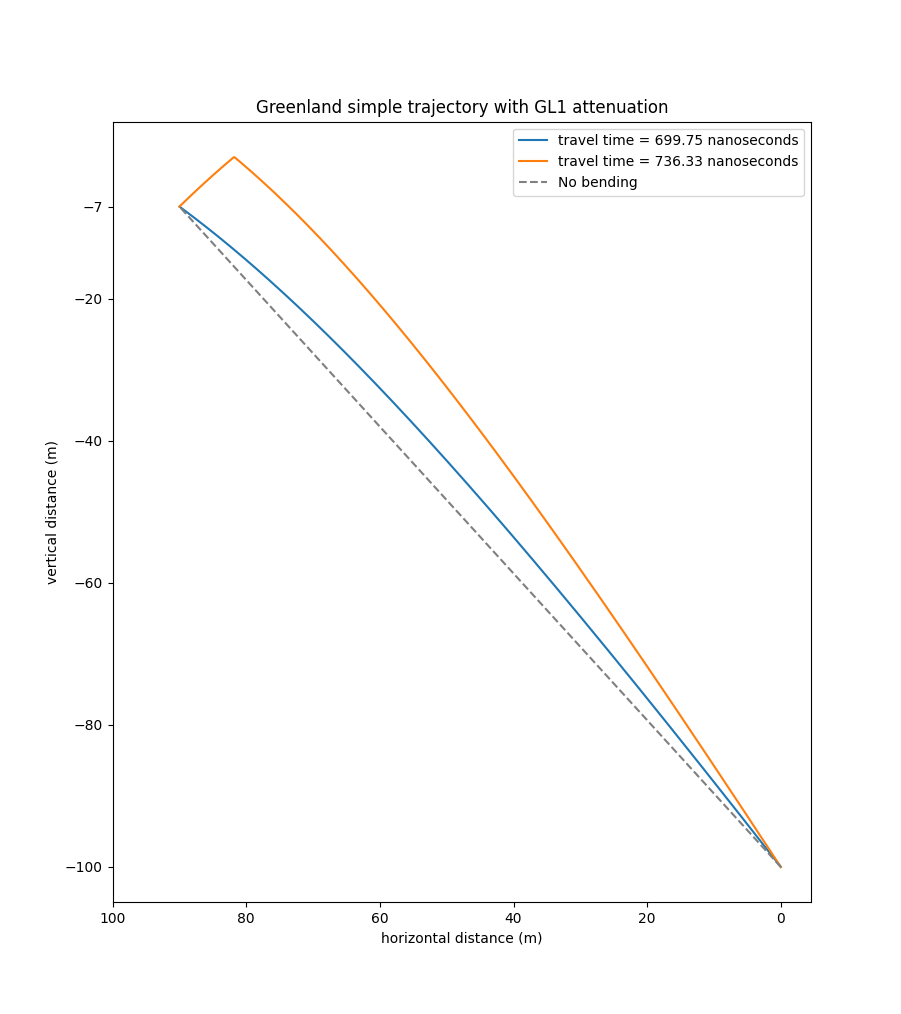
\includegraphics[width=0.8\textwidth]{figures/path_illustration.png}	
	\caption{illustration of a neutrino signal path, the neutrino interaction 
	being located at (0,-100) and the detector at (90,-7)}
	\label{fig:path_illustration}
\end{figure}


This double pulse characteristic would be a smoking-gun signature of an in-ice
source. The two helper strings are needed for a full direction reconstruction.
Three independent measurements are needed for azimuthal information, which is
provided by the Vpol (Vertical polarization) antennas and placing the Hpol
(Horizontal polarization) antennas at different depths on every string, both
zentih and azimuth information will be provided for those signals. The helper
strings' calibration pulsers, as well as one on the surface, will ensure
regular monitoring of the performance of the station and provide information
useful for precise calibration of the antenna geometry.

The plan is to construct these detectors in an array as shown in figure 
\ref{fig:station map}, note that all the individual detectors are named after
various species living in greenland (in the native tongue).

Christoph Welling did an investigation into energy reconstruction from the
received signals\cite{Welling_2019} for air showers in one single station (as
the RNO-G stations are so far apart this is the case here aswell) and he
noticed that it is nescessary to know if the detector who observes an event
falls inside or outside the Cherenkov cone to accurately reconstruct the
primary particle energy as most over-estimated energies in his simulations are
caused by events viewed from within the Cherenkov ring being mistaken for
events outside of it. He went on to show that, if we somehow know if the shower
was seen from inside or outside the ring from some extra source, that most
outliers in the energy disappeared. It is shown by Hiller et
al.\cite{Hiller_2017} that the combination of a muon detector with the radio
detector might make the issue of confusion between being within or outside of
the Cherenkov-ring disappear. Because of this the RNO-G stations are fitted
with surface Log Periodic Dipole Antennas (LPDA), capable of detecting muons.
Note that this is for air showers, the radio signal from neutrinos show
additional complexities.

\begin{figure}
	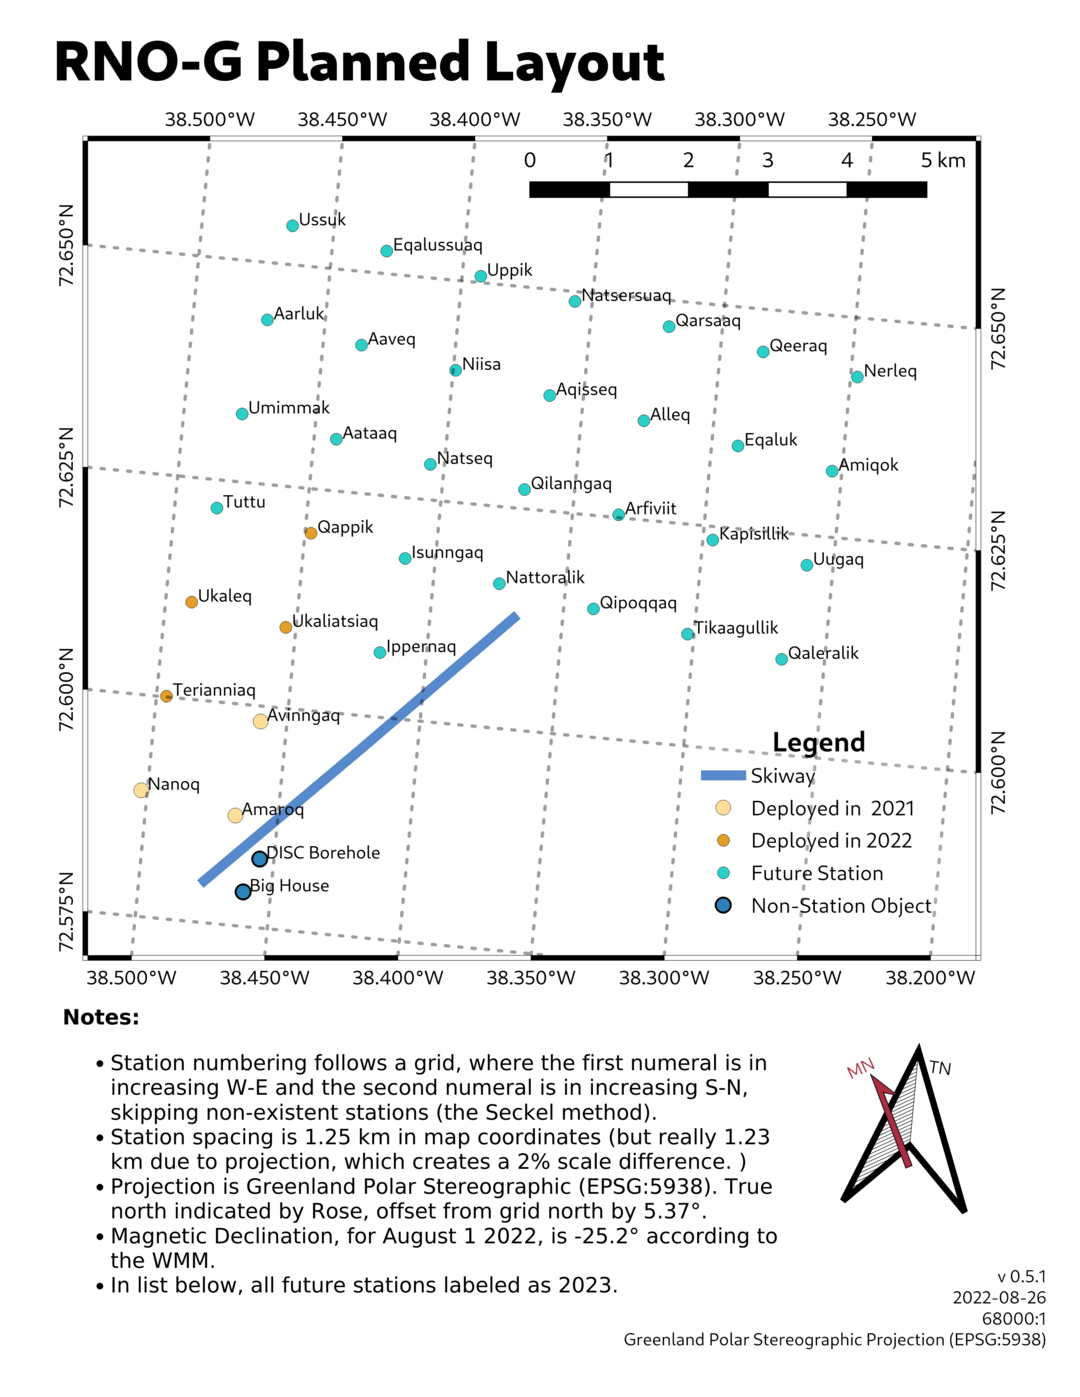
\includegraphics[width=\textwidth]{figures/station-map.png}	
	\caption{map of the station}
	\label{fig:station map}
\end{figure}

\chapter{Hybrid Ray tracer}
%----------------------------------------------------------------------------------------
%	HYBRID RAY TRACER	
%----------------------------------------------------------------------------------------
\section{Shortcomings of the exponential ice model}
It has become apparent (TBC) that complex ice models will be nescessary moving
forward as the exponential ice model fails to fit the density curve.  The ideal
software for radio wave propagation through ice is radiopropa\cite{Winchen_2019}, 
but due to the way it works you'll have to
know the start point , the end point and the launch angle of your ray to work
out the path. This isn't difficult for the analytic model as it's exactly solvable
but for a general ice model you'll somehow have to find where to shoot the ray.
Work has been done on finding the launch angle in the case of complex
ice models by B. Oeyen et al. \cite{2022icrc.confE1027O}, where they
created a ray tracer which iteratively finds the solution, called the
"iterative ray tracer".  The full explanation of how their algorithm works can
be found in the mentioned paper.  This is however a sub-optimal solution in
python as an optimalisation library will generally work faster, work had been
done on trying to implement such an algorithm but this attempt failed.  As we
saw this work the idea came to mind to combine the iterative ray tracer and the code
using the optimisation libraries (a so called "minimizer"), to come up with the
algorithm that will be discussed in this chapter: The hybrid ray tracer, in the
source code called the "hybrid minimizer".

It succeeds in more rapidly tracing the path from the event to the detector, is
more accurate and also arrives closer to the detector as the final result is
not limited by the final drawn sphere size but by a given tolerence.

\section{How it works}
The full code can be found in appendix \ref{chapter: Hybrid minimizer code},
here we'll walk you through the algorithm.  The hybrid minimizer can be seen as
an extension of the iterative raytracer \cite{2022icrc.confE1027O} as it starts
out the same way: Say our source of radiation is at position $\mathbf{X}_1$ and
our detector is located at position $\mathbf{X}_2$, we start by defining the
vector $\mathbf{v} = \mathbf{X}_2 - \mathbf{X}_1$, then we clone it as a new
vector u and set u's z coordinate to 0, making it a normal vector of a plane
parallel to the z direction. we now wish to know where we'd actually be able to
find possible paths, looking at figure \ref{fig:path_illustration} we see that
no solutions below the direct path are possible as there would need to be
upwards reflection, so we convert our vector $\mathbf{v}$ representing the path
from the source to the detector to spherical coordinates, giving us a polar
angle (zenith angle) "theta-direct". With this we know that the, at the source,
the ray should propagate with an initial zenith angle within the angle interval
0° to theta-direct° $:= \Omega$.

Next we need to define our "observers", if you shoot a ray with the radiopropa module from a certain
point at a certain angle the ray path will get simulated until it interacts with this "observer".
Ideally we would like to a priori know where to shoot our ray and have the detector be an infinitesimally small
observer in our simulation, but as we'll be working with general ice models this can't be done.

The algorithm of finding the possible paths is then as follows:
We define a spherical observer at the location of the detector, with a radius of fair size. We place an 
observer plane directly behind the detector (with normal vector $\mathbf{u}$, no rays can propagate back after crossing) 
and an observer above the surface (as no rays could make it back after escaping the ice) our 
full setup is then what's illustrated in the figure below
\begin{figure}[h!]
  \centering
  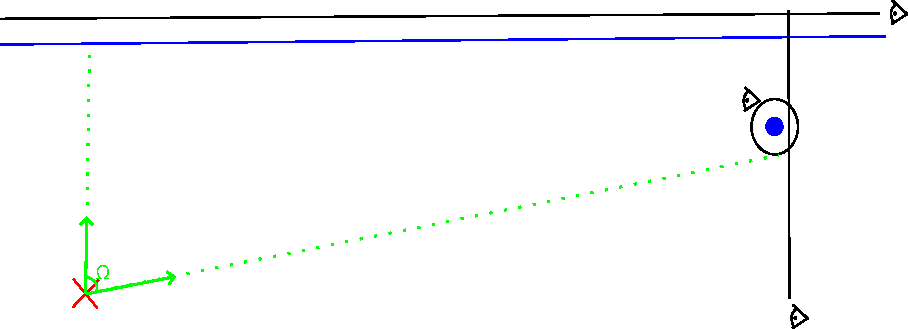
\includegraphics[width=0.6\textwidth]{algoillu.pdf}
\end{figure}\\

Here the red cross is the radio source, the blue horizontal line is the ice-air
boundary surface, the blue dot to the right is the detector and the green
$\Omega$ indicates the range over which solutions to the problem are possible.

We start off by just iteratively guessing: given a certain angle stepsize $\Delta \theta$ shoot rays
at the angles $\{0,\Delta \theta, 2\Delta \theta,...,\Omega\}$ And see which ones get detected 
at the sphere around the detector, this process is illustrated in a modified version of B. Oeyen
et al. their figure below\\
\begin{figure}[h!]
  \centering
  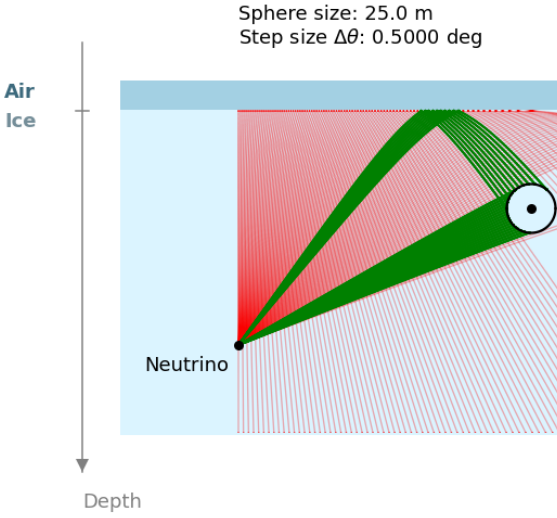
\includegraphics[width=0.5\textwidth]{begin_explanation.png}
\end{figure}\\
if there are 2 distinct launch regions, it will start the so called "minimization", using scipy's module 
optimize.minimize. First we get rid of the spherical observer and place the vertical observer exactly at
the detector, now
to be able to use the minimize module we'll need a function to minimze, for this reason we define the function 
\textit{delta\_z} as, given a certain launch angle, returning the distance from the point where it lands on the
plane to the detector as illustrated below
\begin{figure}[h!]
  \centering
  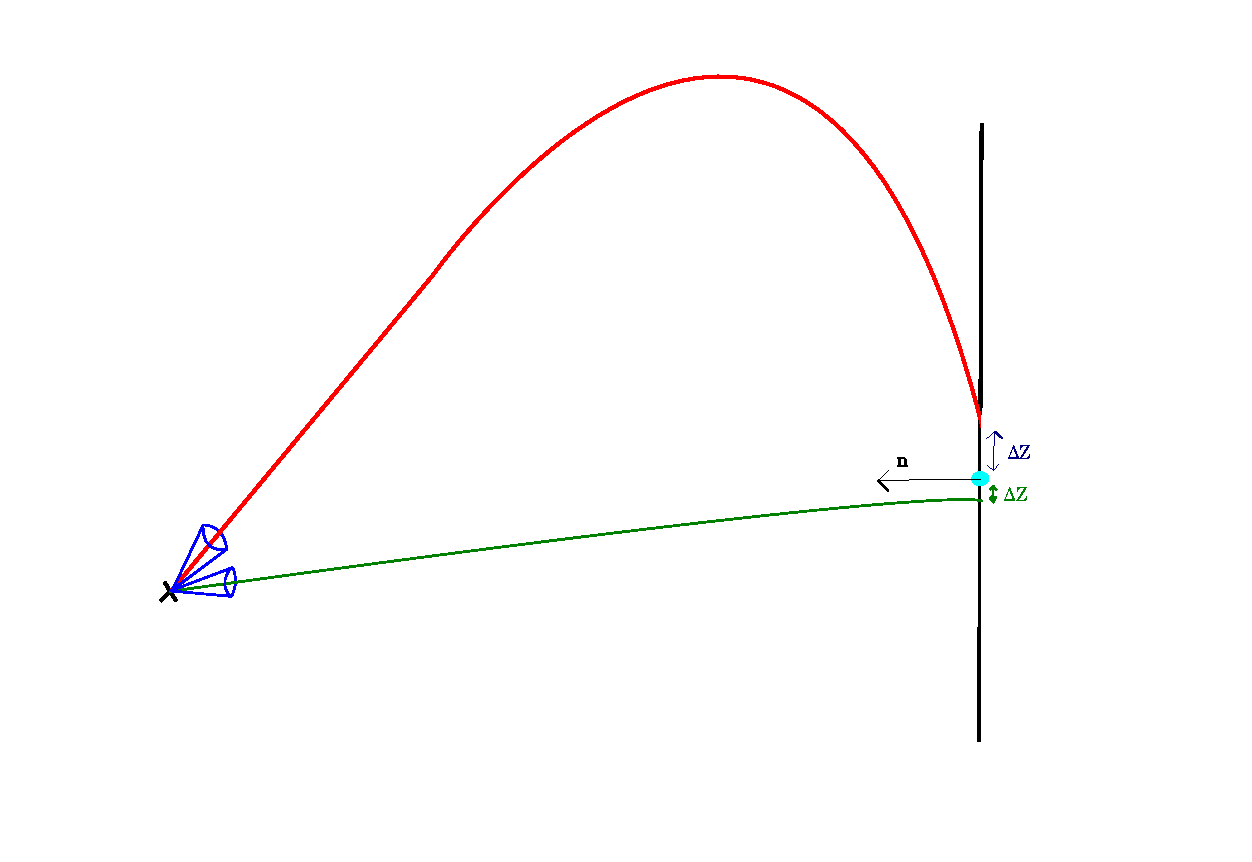
\includegraphics[width=0.5\textwidth]{PrincipleHybridIllu.pdf}
\end{figure}\\
The function we'll minimize is then detla\_z\_squared which is just the square of delta\_z as we wish it to be
as close as possible to 0, it gets minimized within the angle boundaries found from the previous step.
With this our algorithm is done, it does have a fail-safe as well for if the first step, finding the launch
regions, doesn't work namely it reverts back to being the iterative ray tracer.
\section{Performance Optimalisation}
To test the hybrid minimizer the numpy random module was used to generate
random coördinates, the considered square (as there is only a z component to the
ice model the 3D problem is essentially only a 2D problem) is x:0.1km,4km and
z:-0.1km,-3km.\footnote{This start at 100m depth was to get around issues concerning events that 
won't even trigger in a full simulation}
Every test point shown in the following subsections consists of at least 500 random initial positions.
As the speed of the algorithm is computer dependent the algorithm's speed is always plotted relative to
the iterative ray tracer's speed, simulated with the same coordinates at the same time.
\subsection{Length of the normal vector}
\begin{figure}[h!]
	\centering
	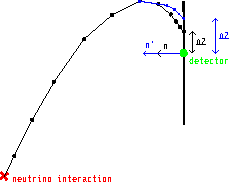
\includegraphics[width=0.7\textwidth]{figures/PrincipleNormIllu.pdf}
	\caption{how normal vector size influences the stepsize}
	\label{fig:normexpl}
\end{figure}
As visually explained in figure \ref{fig:normexpl}, the size of the normal vector seems to
influence how big the ray tracer's step size is taken close to the detector. This
thus influences the convergence and time taken. The results of varying this are shown
in figures \ref{fig:norminfl} and \ref{fig:norminfl2}.
Looking at these figures the first optimization conclusion is as expected: 
take the normal vector length to be 1 meter.
\subsection{ztol}
We'll now change the tolerence on the vertical distance away from the detector which is deemed
accepted i.e in figure \ref{fig:normexpl} if $\Delta z$ is below this threshold it's accepted.
The results are shown in figures \ref{fig:ztolinfl} and \ref{fig:ztolinfl2}.
From which we can conclude the second optimization conclusion: take ztol to be 0.05 m.
\subsection{Sphere Size \& Step Size}
The initial rays are sent out in steps of a certain angle and with a sphere
around the detector of a certain size. As this initial search for launch angle
regions is the slowest step in the hybrid ray tracer it's imperative to
optimize this. The procedure was: change the sphere size and loop over various
step sizes, recording the speed. The results are shown in figure \ref{fig:SphereStepInfl} 
the lower on the chart the better, zooming in onto the lowest point as is shown in a combined
plot on figure \ref{fig:SphereStepFinal}, we see that an optimum seems to be around a spheresize
of 45m and a stepsize of 0.7°.

\begin{figure*}
	\centering
\begin{minipage}{0.49\textwidth}
	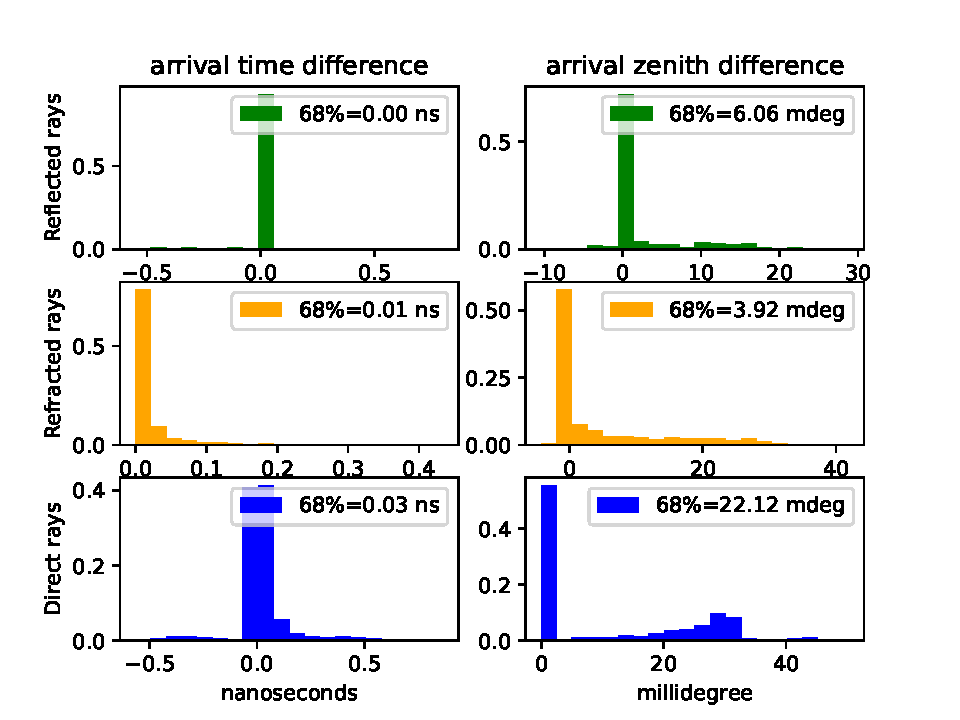
\includegraphics[width=1.1\textwidth]{figures/hybrid_comparison_N_1000.pdf}
	\caption{Hybrid}
	\label{fig:acchyb}
\end{minipage}
\begin{minipage}{0.49\textwidth}
	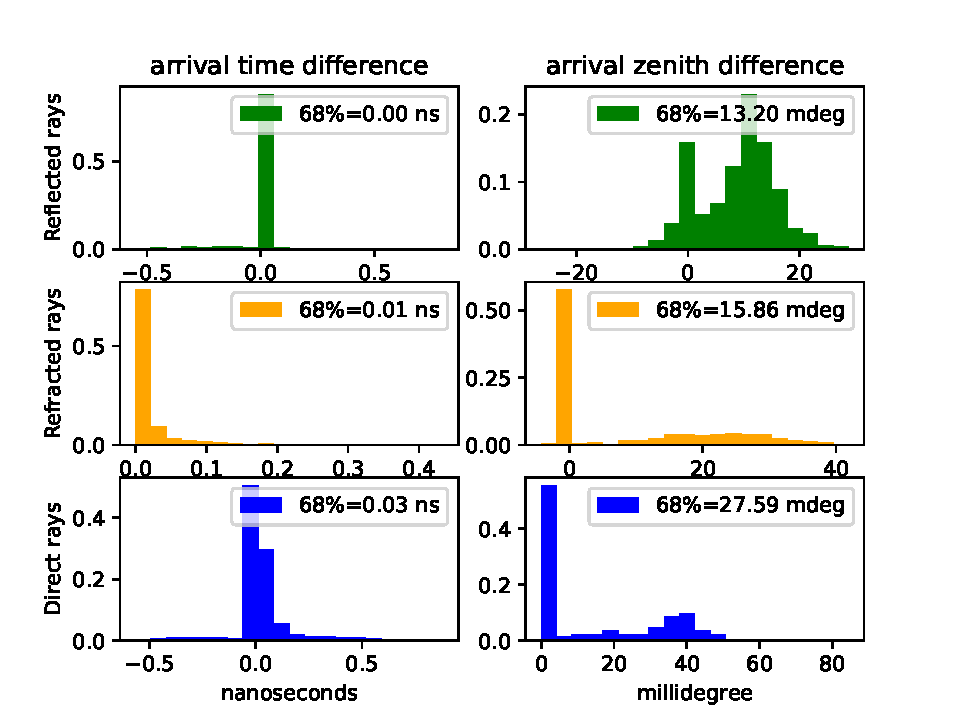
\includegraphics[width=1.1\textwidth]{figures/iterative_comparison_N_1000.pdf}
	\caption{Iterative}
	\label{fig:accit}
\end{minipage}
\end{figure*}

\begin{figure}
	\centering
	\begin{minipage}{\textwidth}
		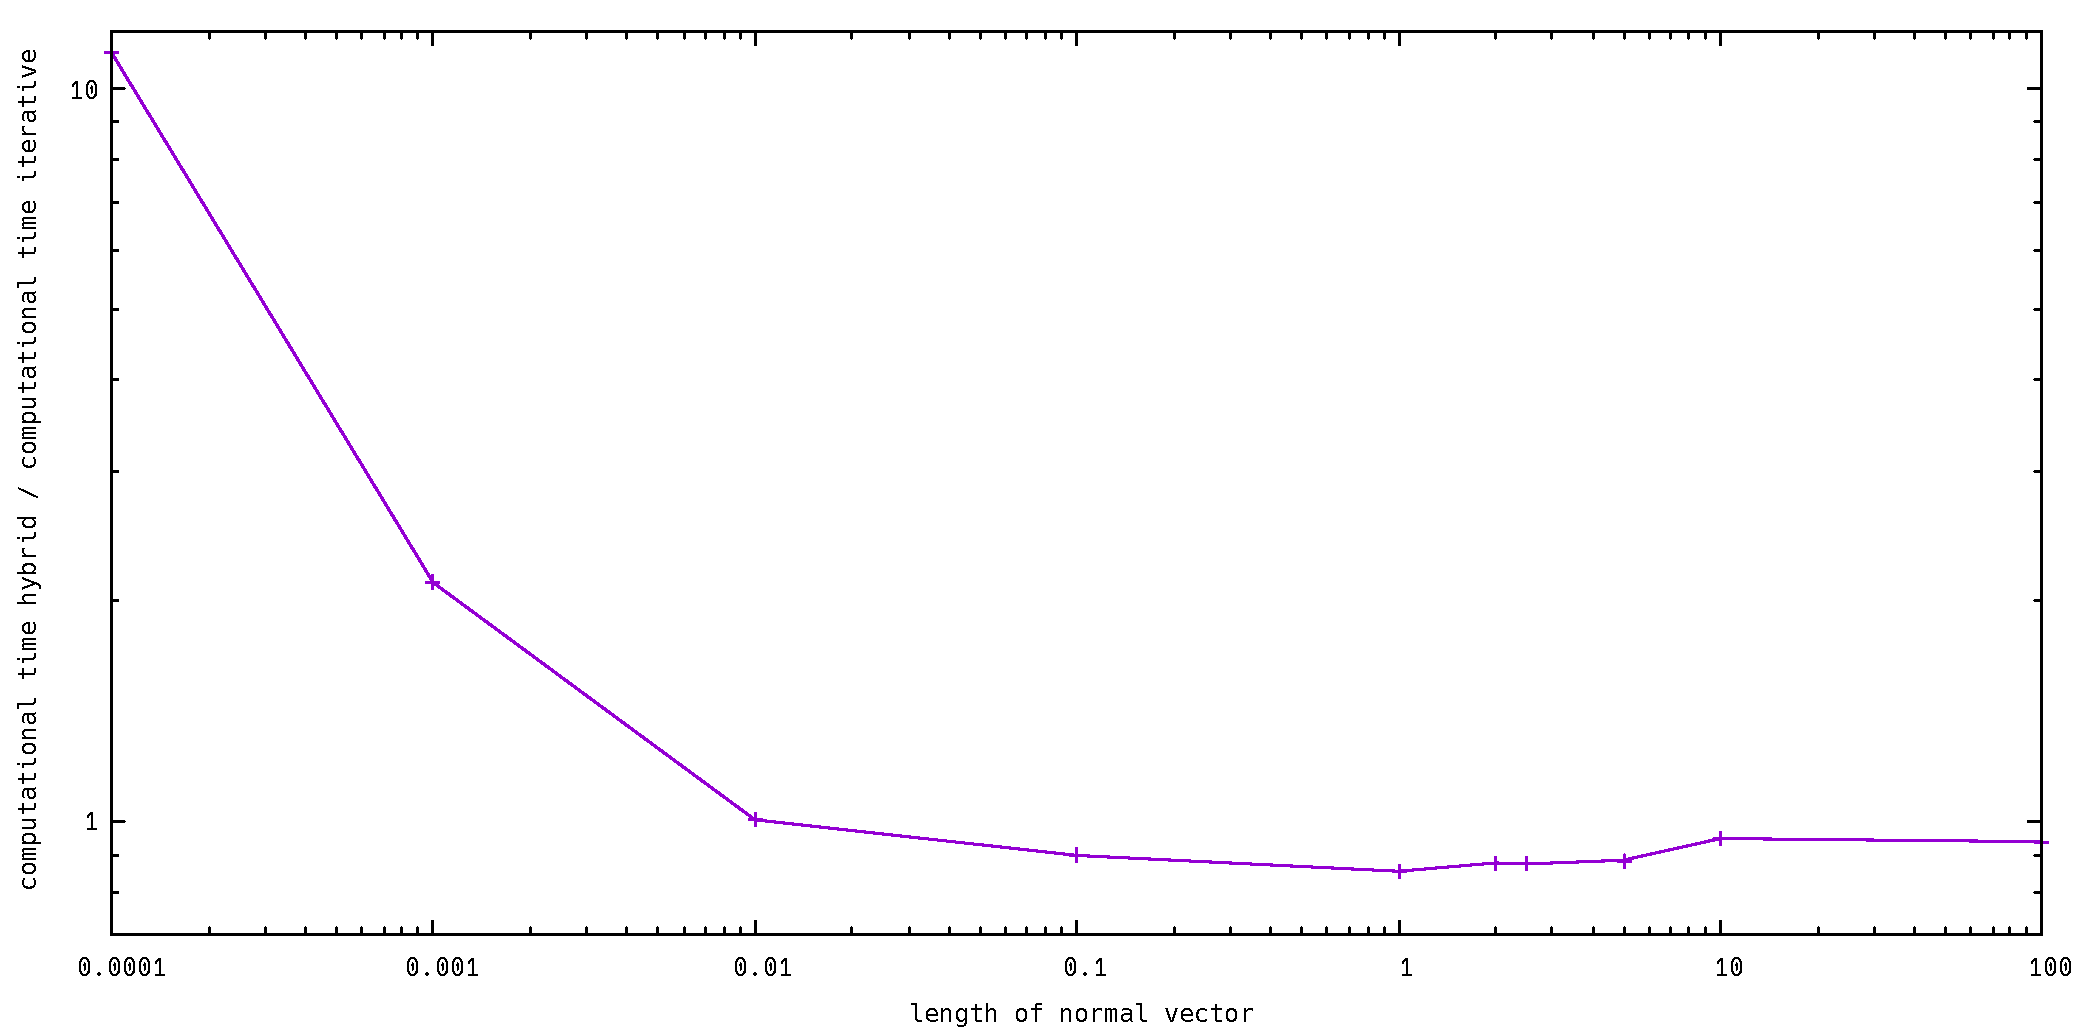
\includegraphics[width=0.8\textwidth]{figures/NormVsTime.pdf}
	\end{minipage}
	\begin{minipage}{\textwidth}
		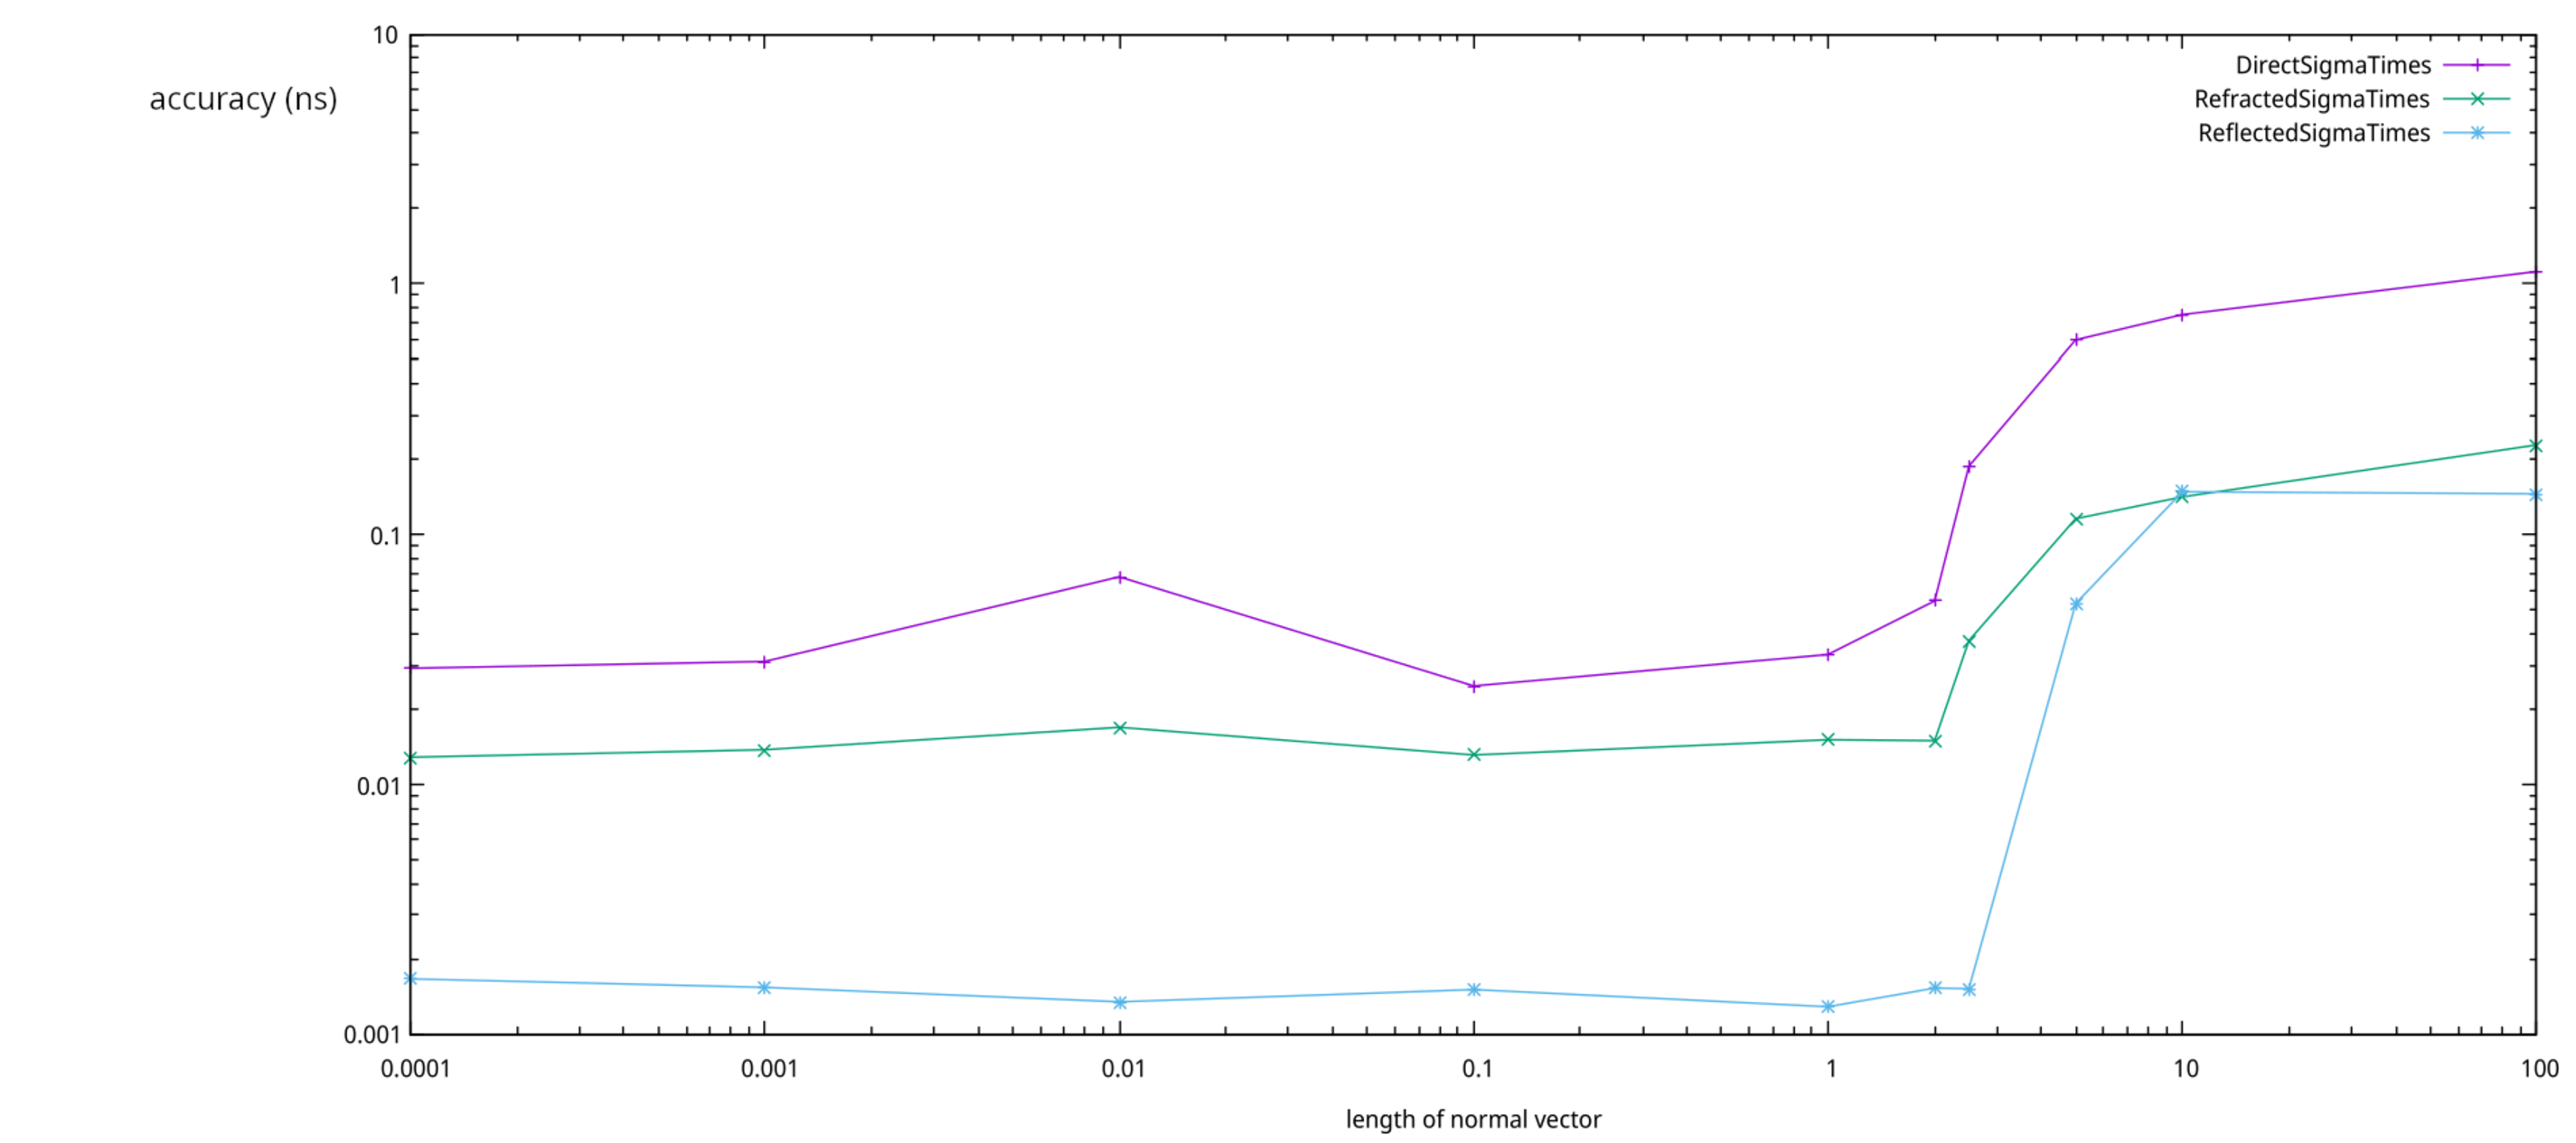
\includegraphics[width=0.8\textwidth]{figures/NormVsSigmaTime.pdf}
	\end{minipage}
\caption{influence of the length of the normal vector}
\label{fig:norminfl}
\end{figure}
\begin{figure}
	\centering
	\begin{minipage}{\textwidth}
		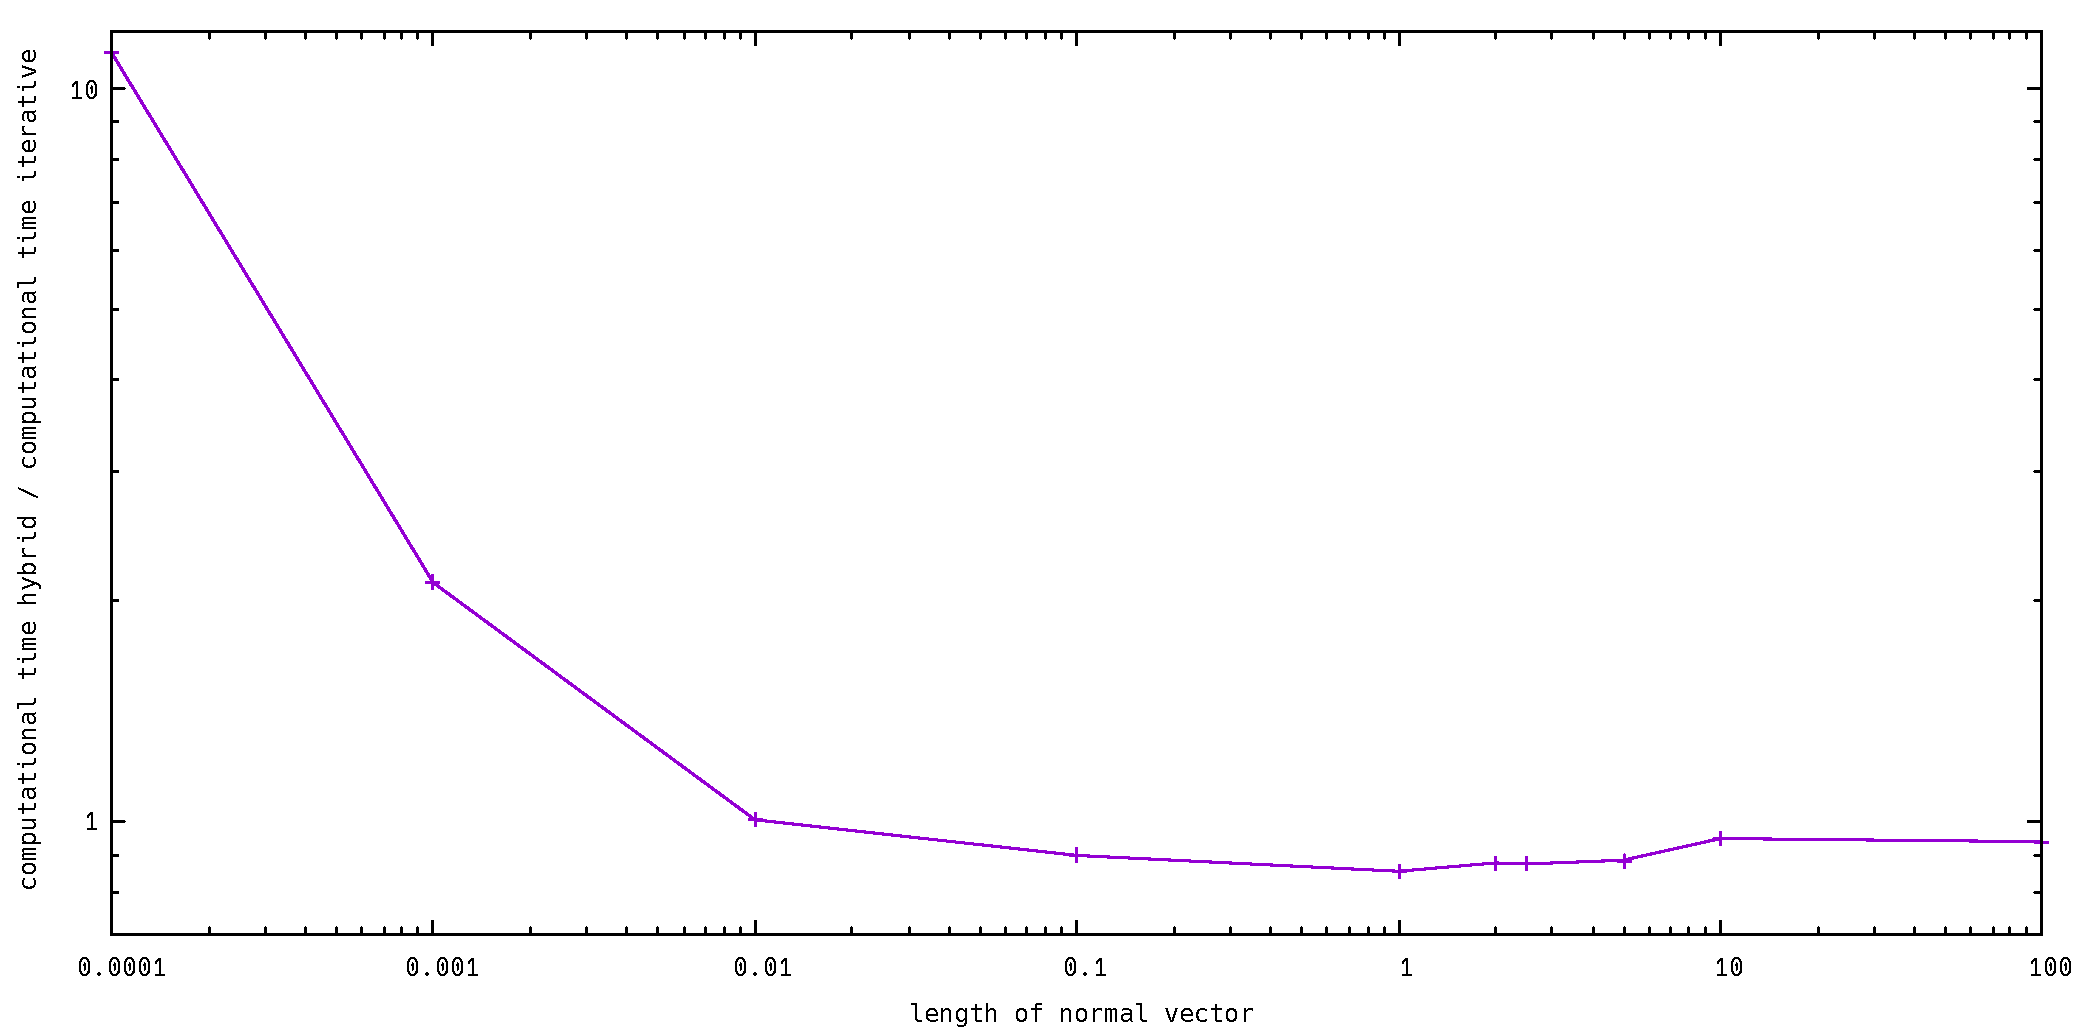
\includegraphics[width=0.8\textwidth]{figures/NormVsTime.pdf}
	\end{minipage}
	\begin{minipage}{\textwidth}
		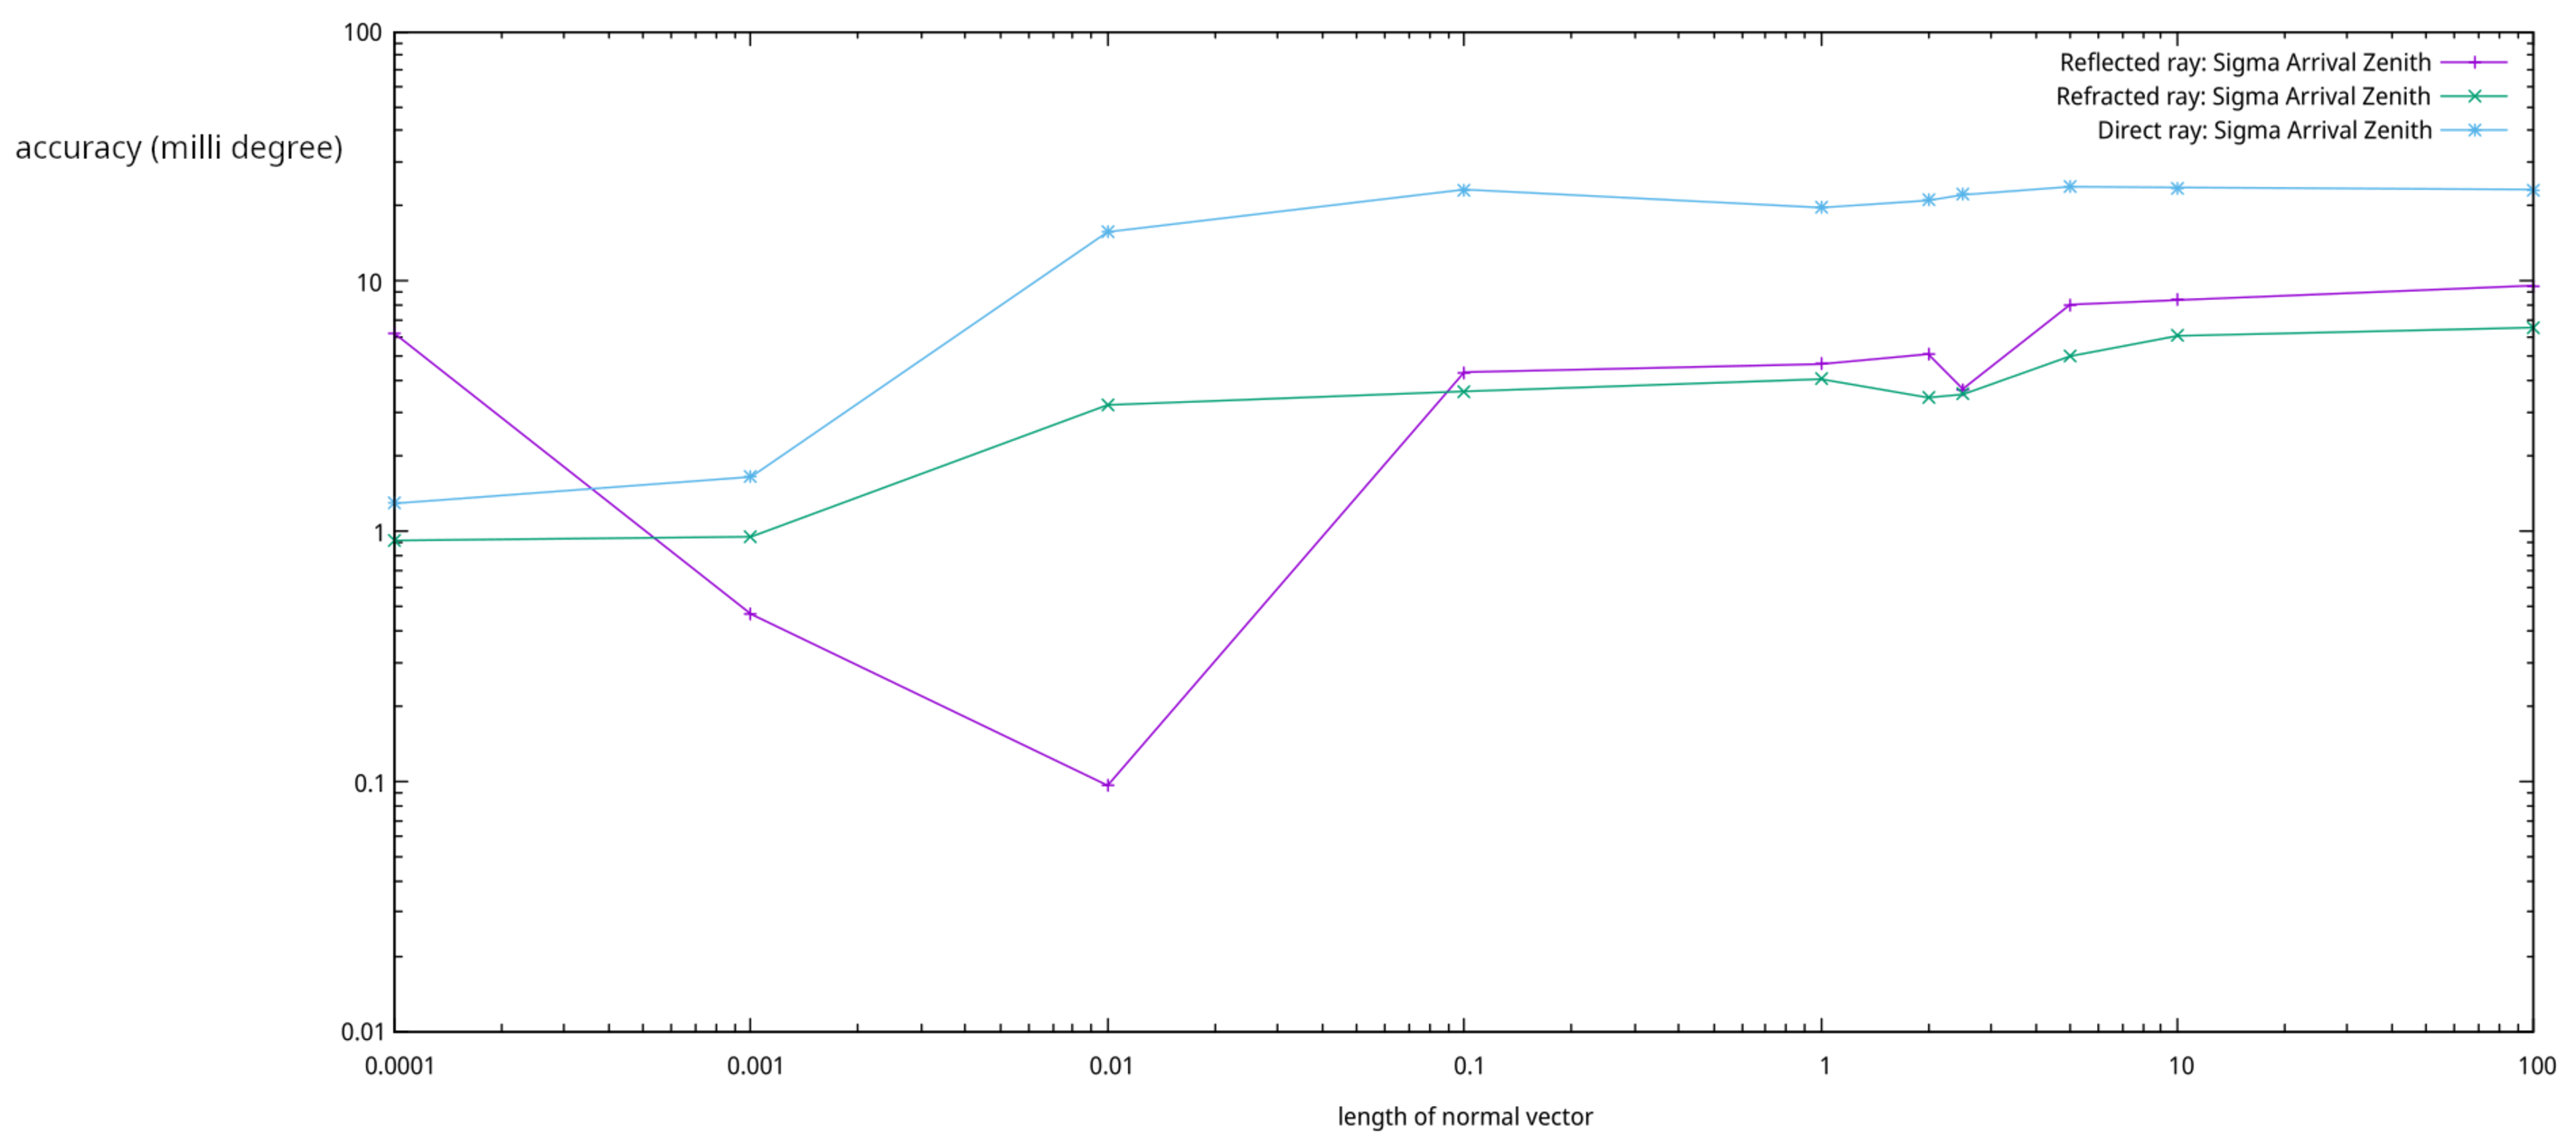
\includegraphics[width=0.8\textwidth]{figures/NormVsSigmaAZ.pdf}
	\end{minipage}
\caption{influence of the length of the normal vector}
\label{fig:norminfl2}
\end{figure}

\begin{figure}
	\centering
	\begin{minipage}{\textwidth}
		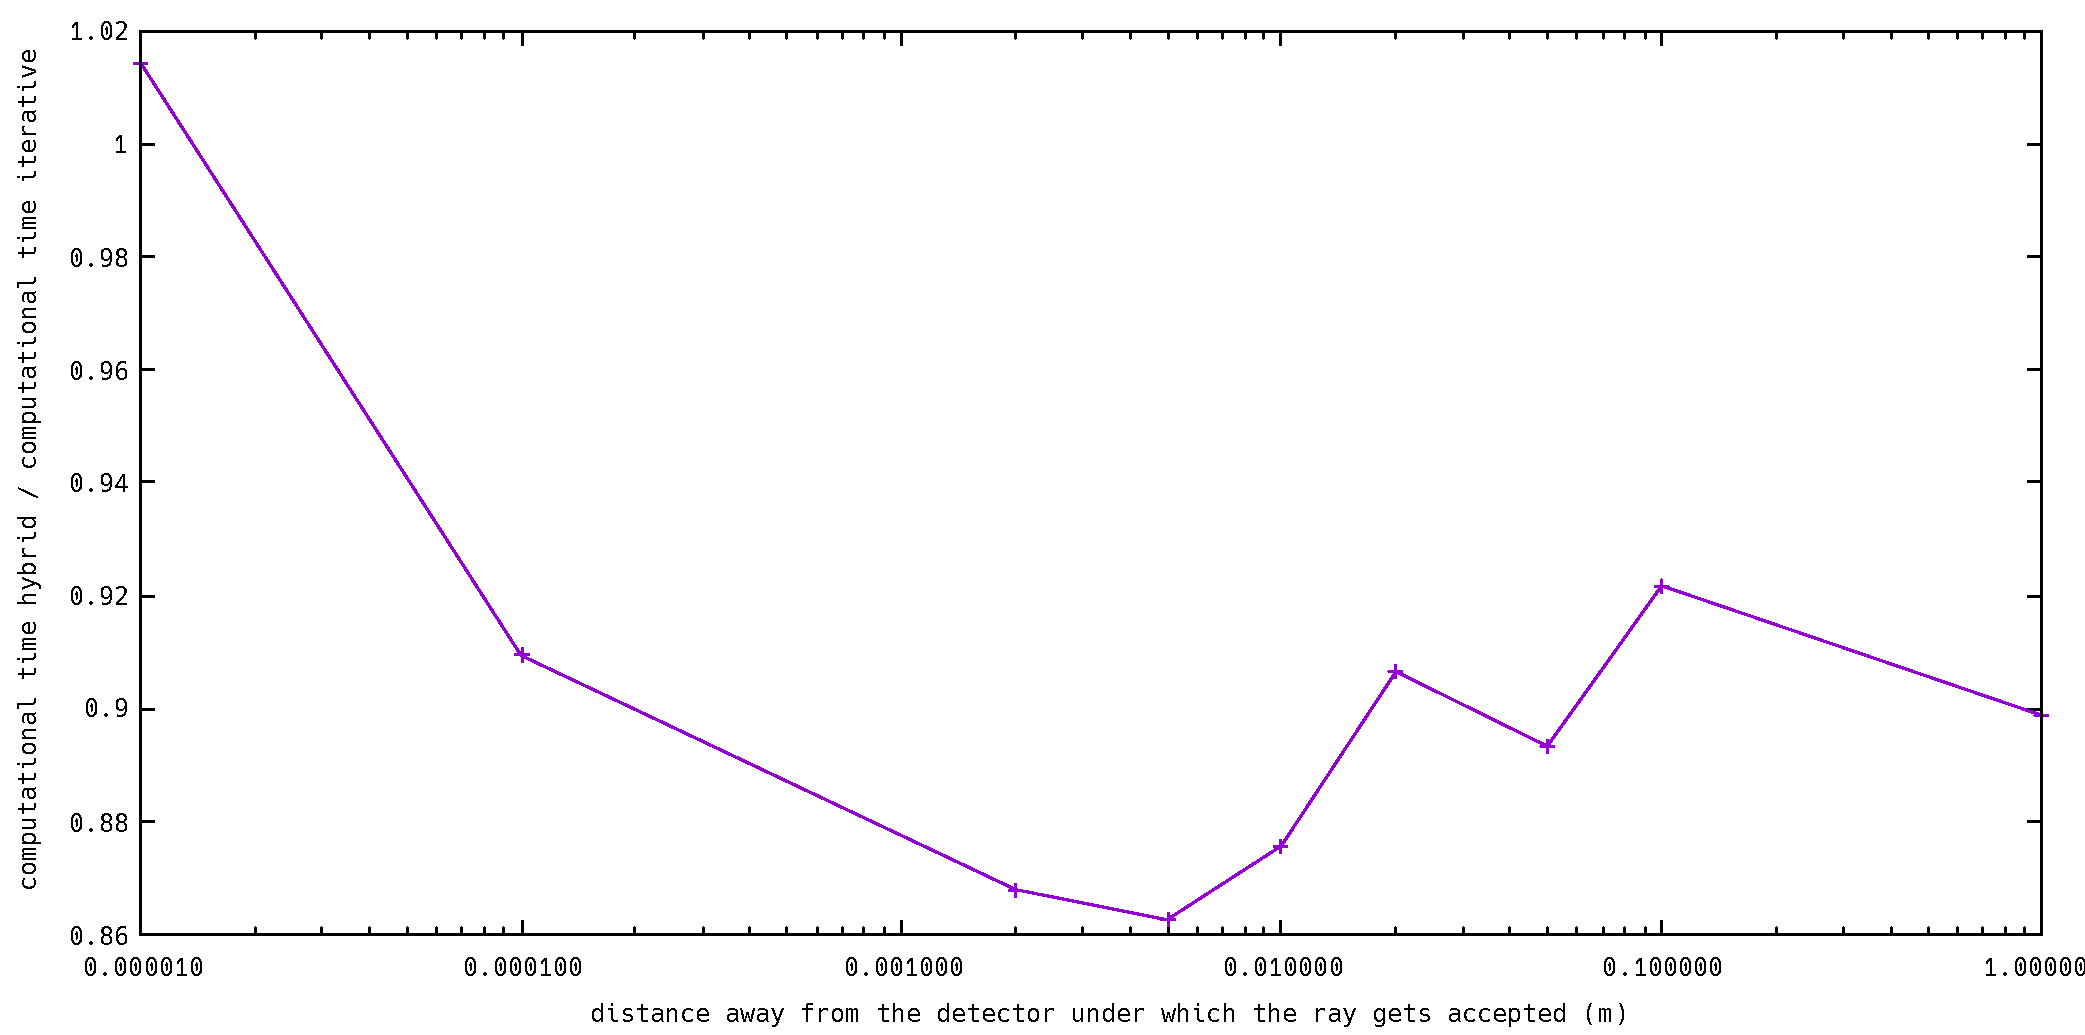
\includegraphics[width=0.8\textwidth]{figures/ZtolVsTime2.pdf}
	\end{minipage}
	\begin{minipage}{\textwidth}
		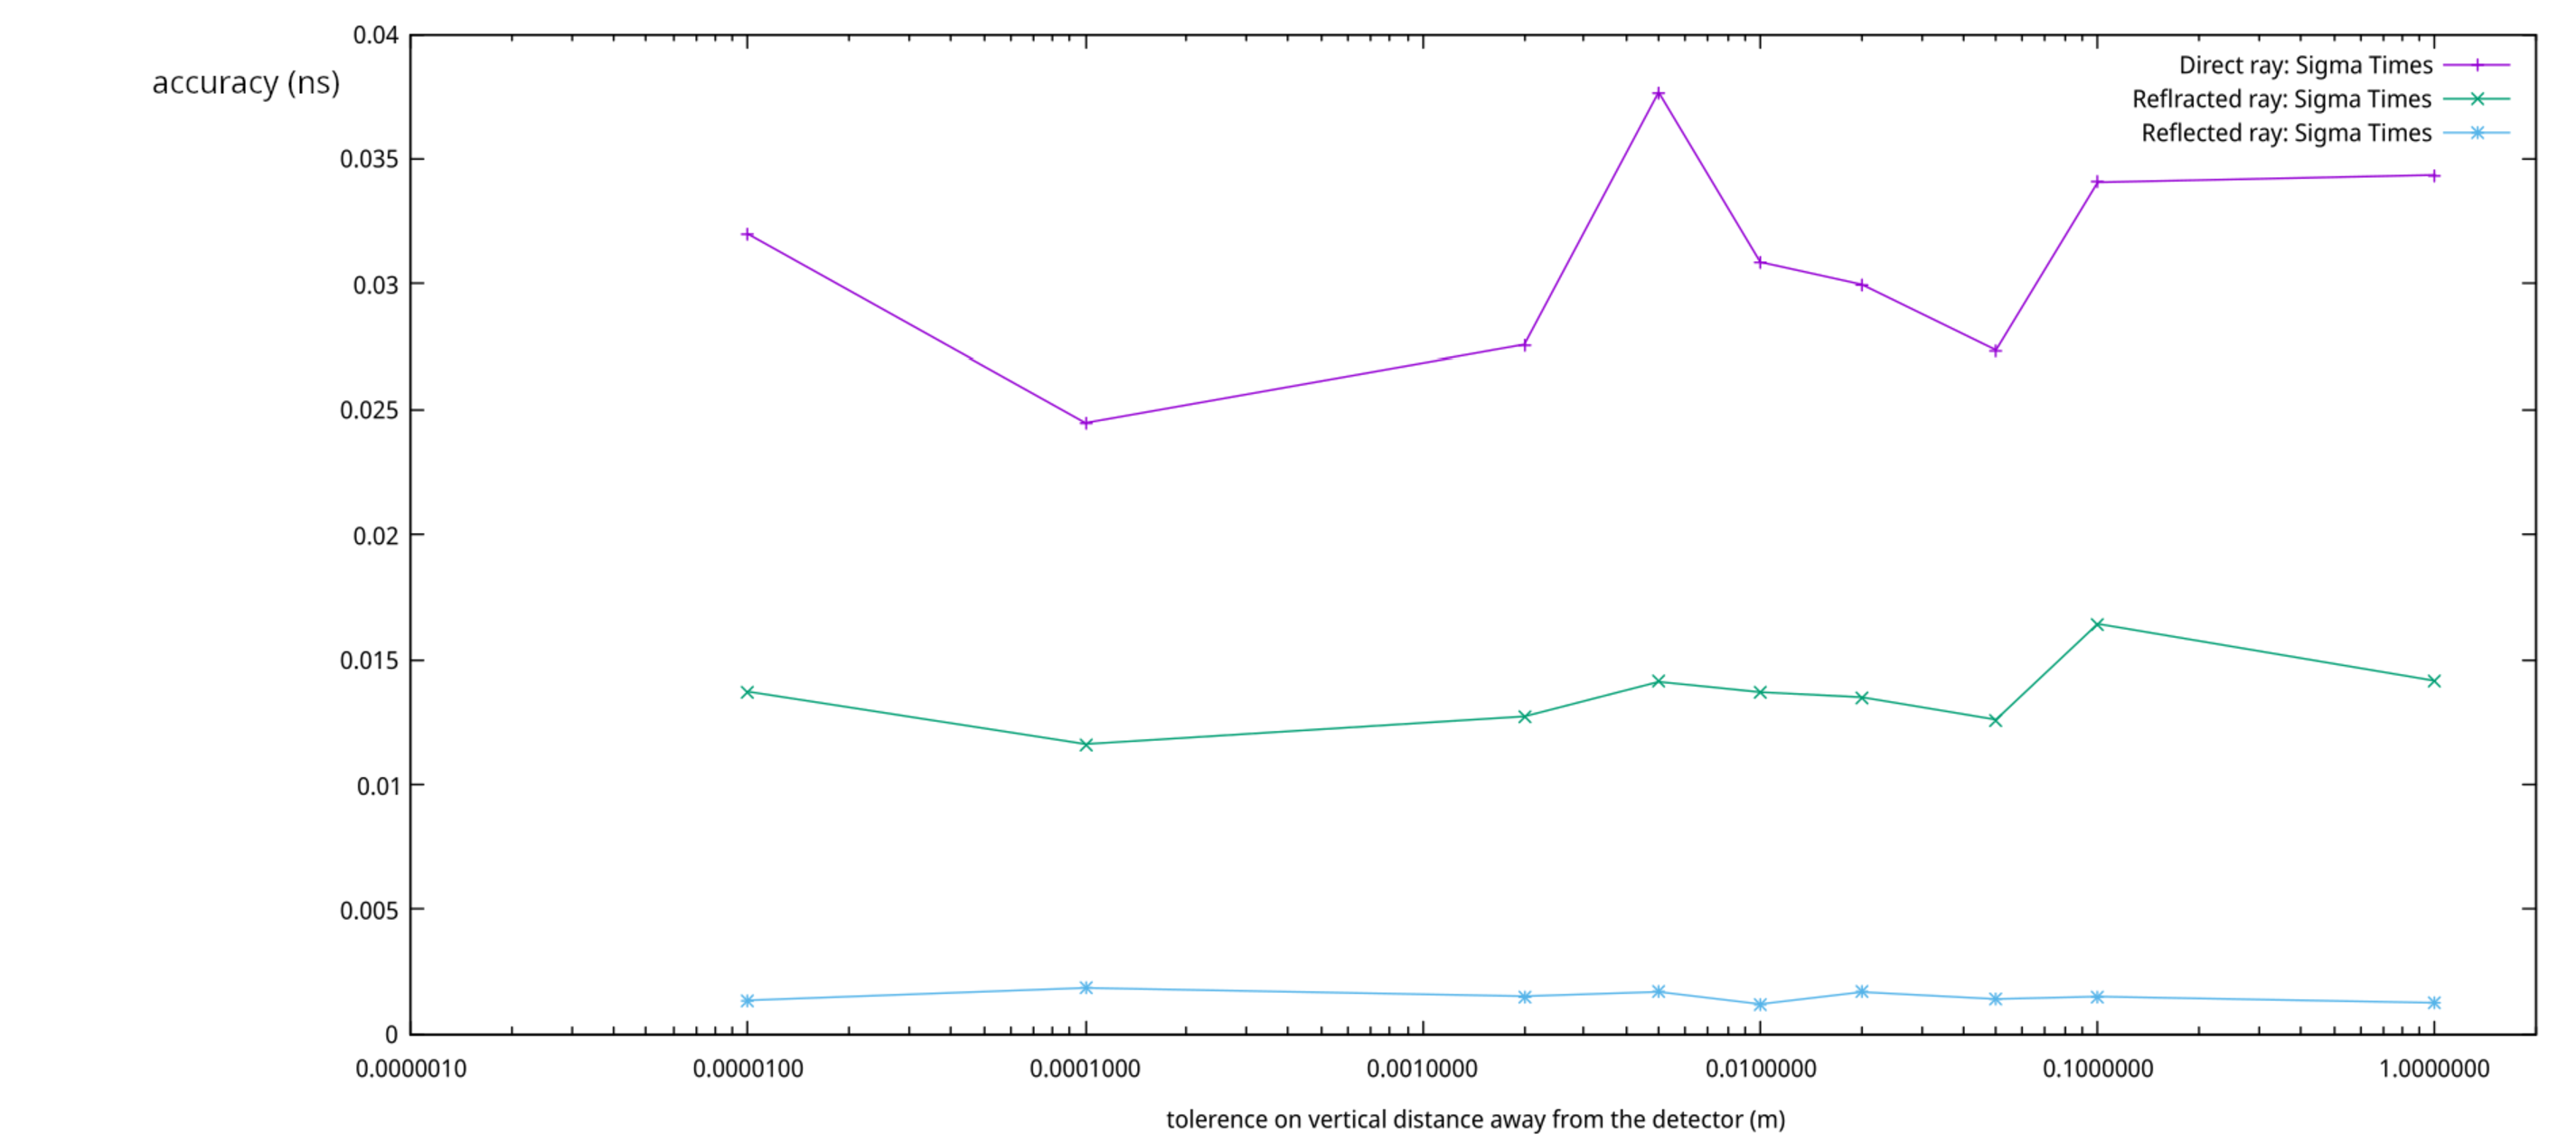
\includegraphics[width=0.8\textwidth]{figures/ZtolVsSigmaTime.pdf}
	\end{minipage}
\caption{influence of the tolerence on vertical distance}
\label{fig:ztolinfl}
\end{figure}

\begin{figure}
	\centering
	\begin{minipage}{\textwidth}
		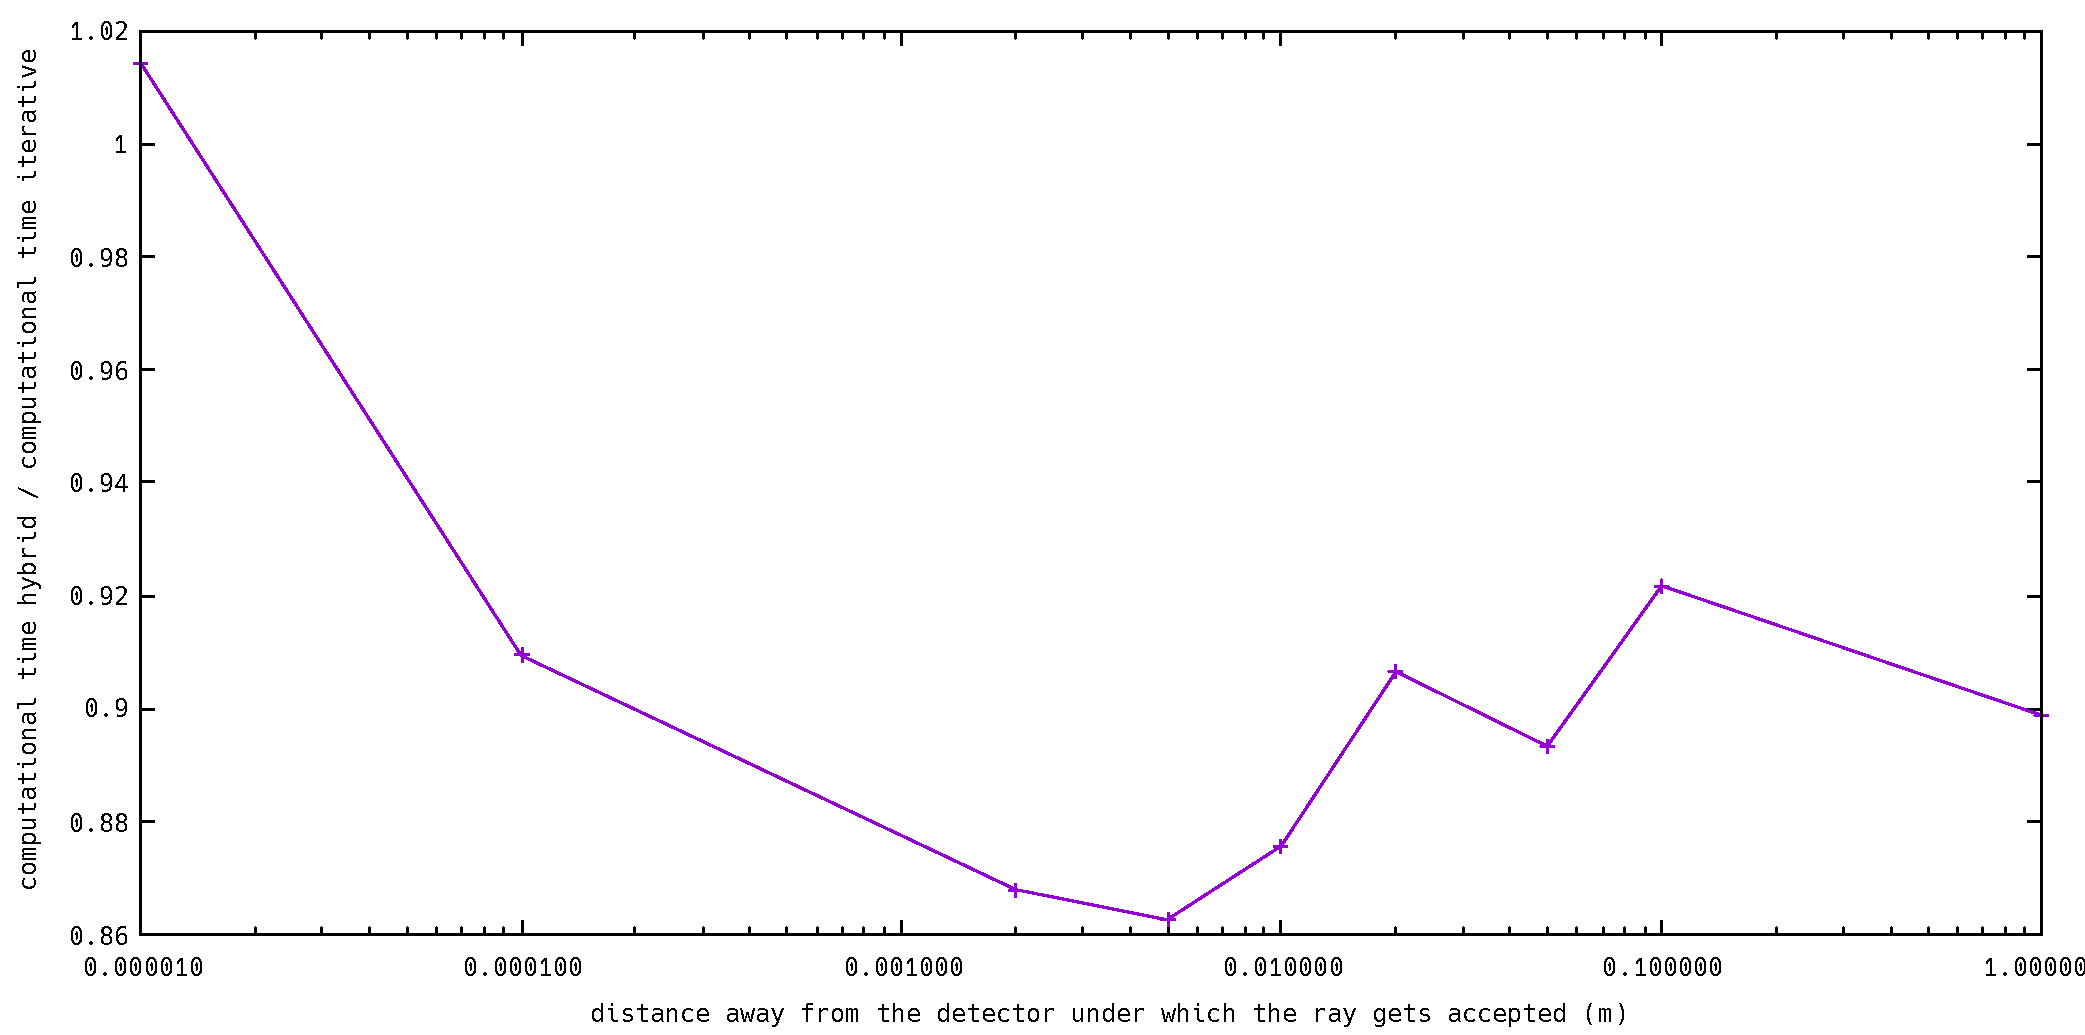
\includegraphics[width=0.8\textwidth]{figures/ZtolVsTime2.pdf}
	\end{minipage}
	\begin{minipage}{\textwidth}
		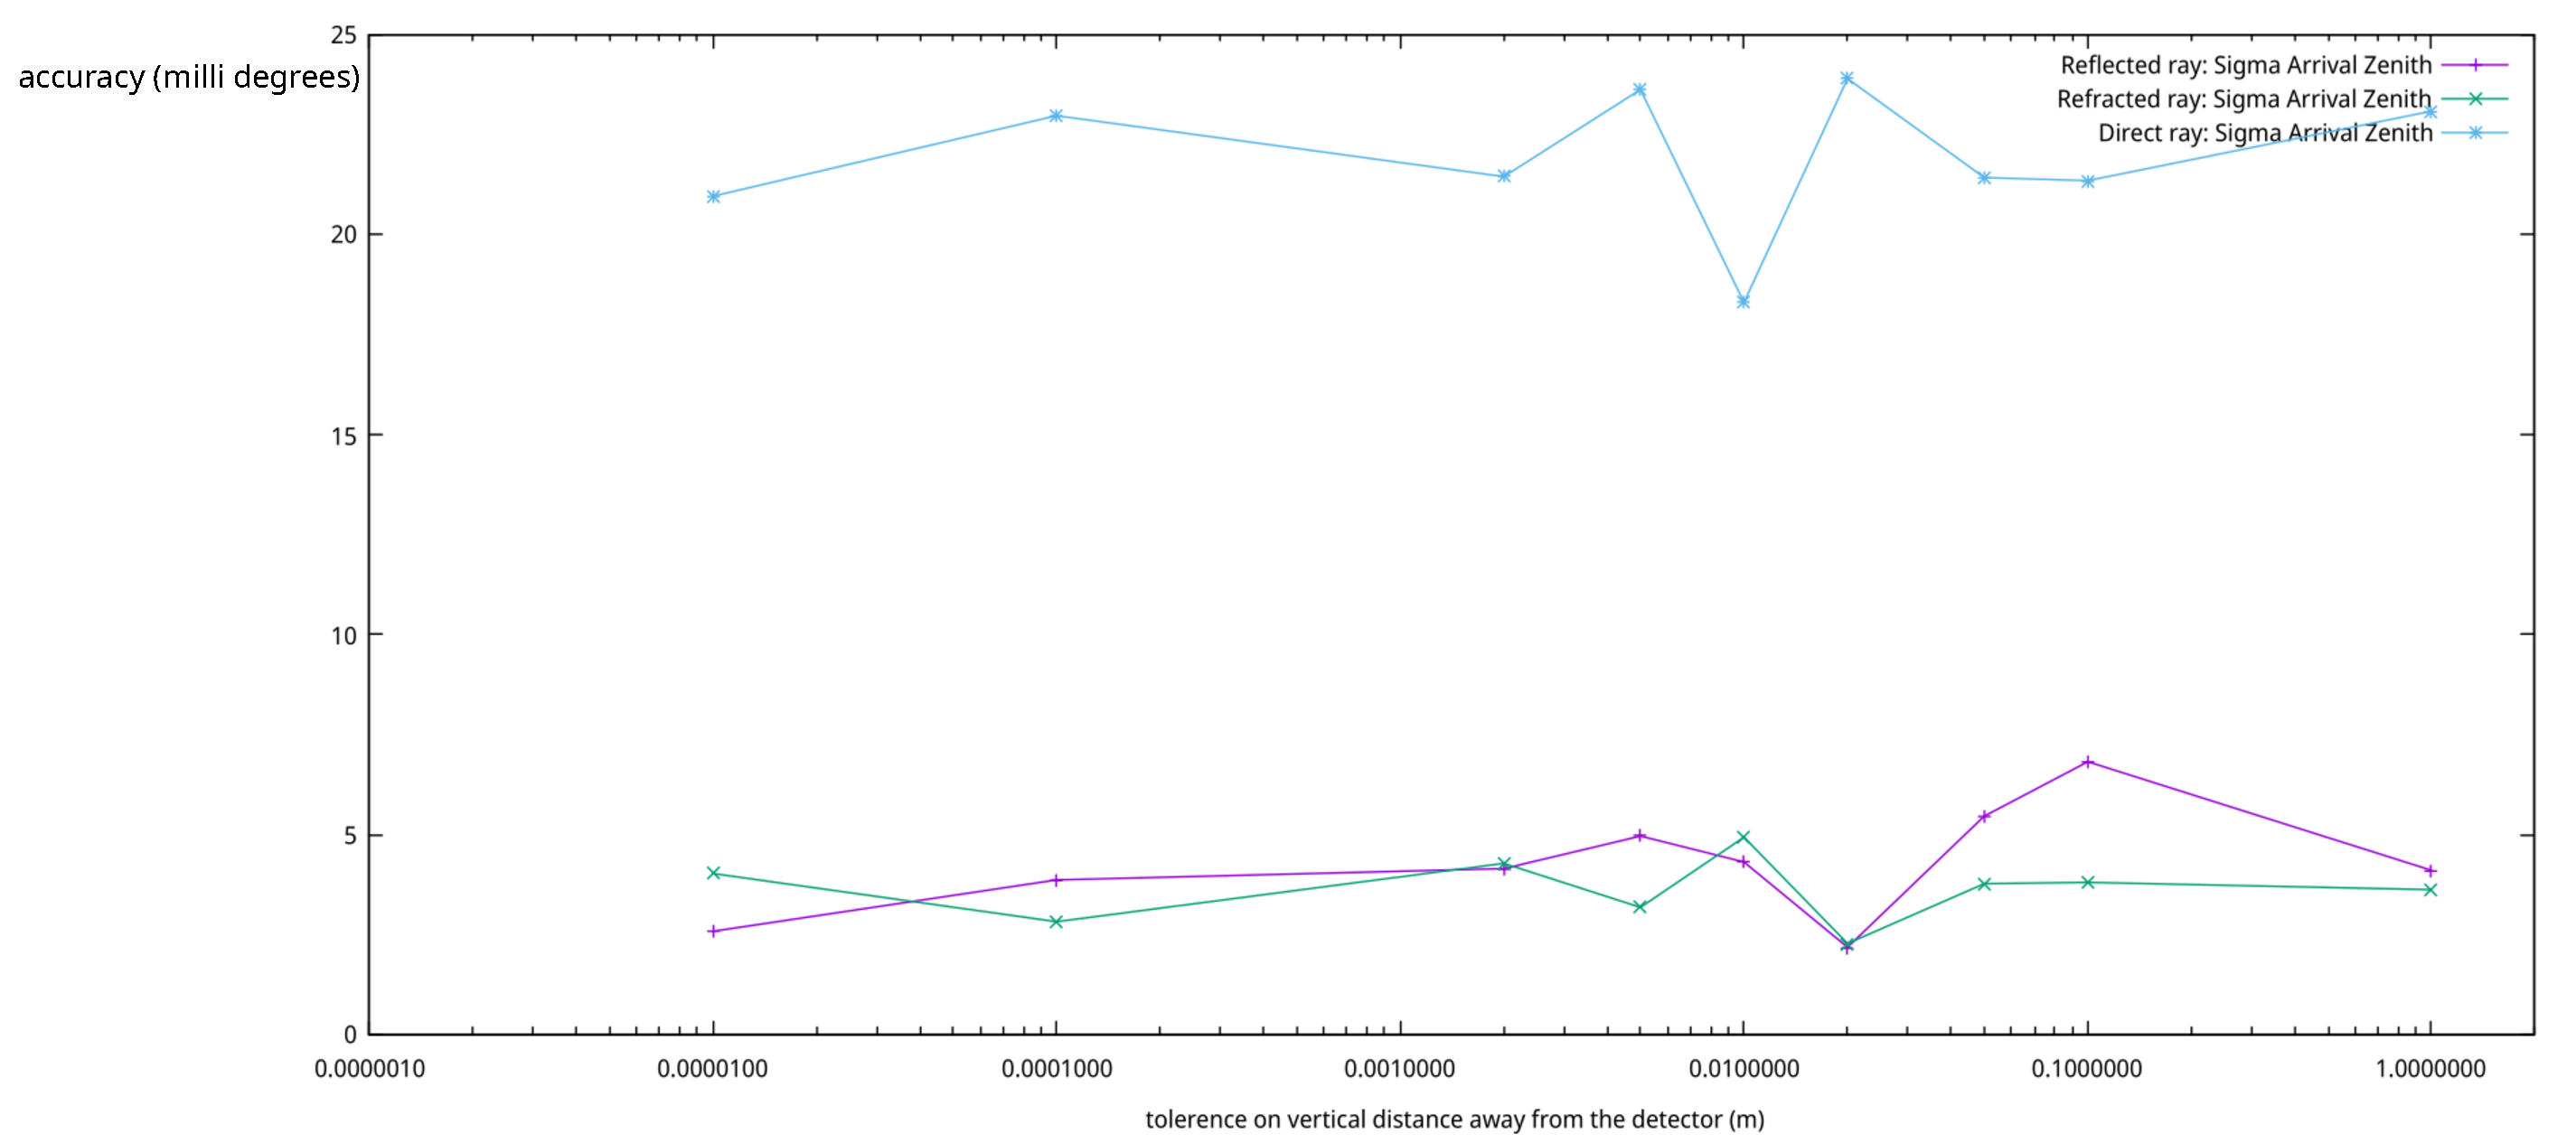
\includegraphics[width=0.8\textwidth]{figures/ZtolVsSigmaAZ.pdf}
	\end{minipage}
\caption{influence of the tolerence on vertical distance}
\label{fig:ztolinfl2}
\end{figure}

\begin{figure}
	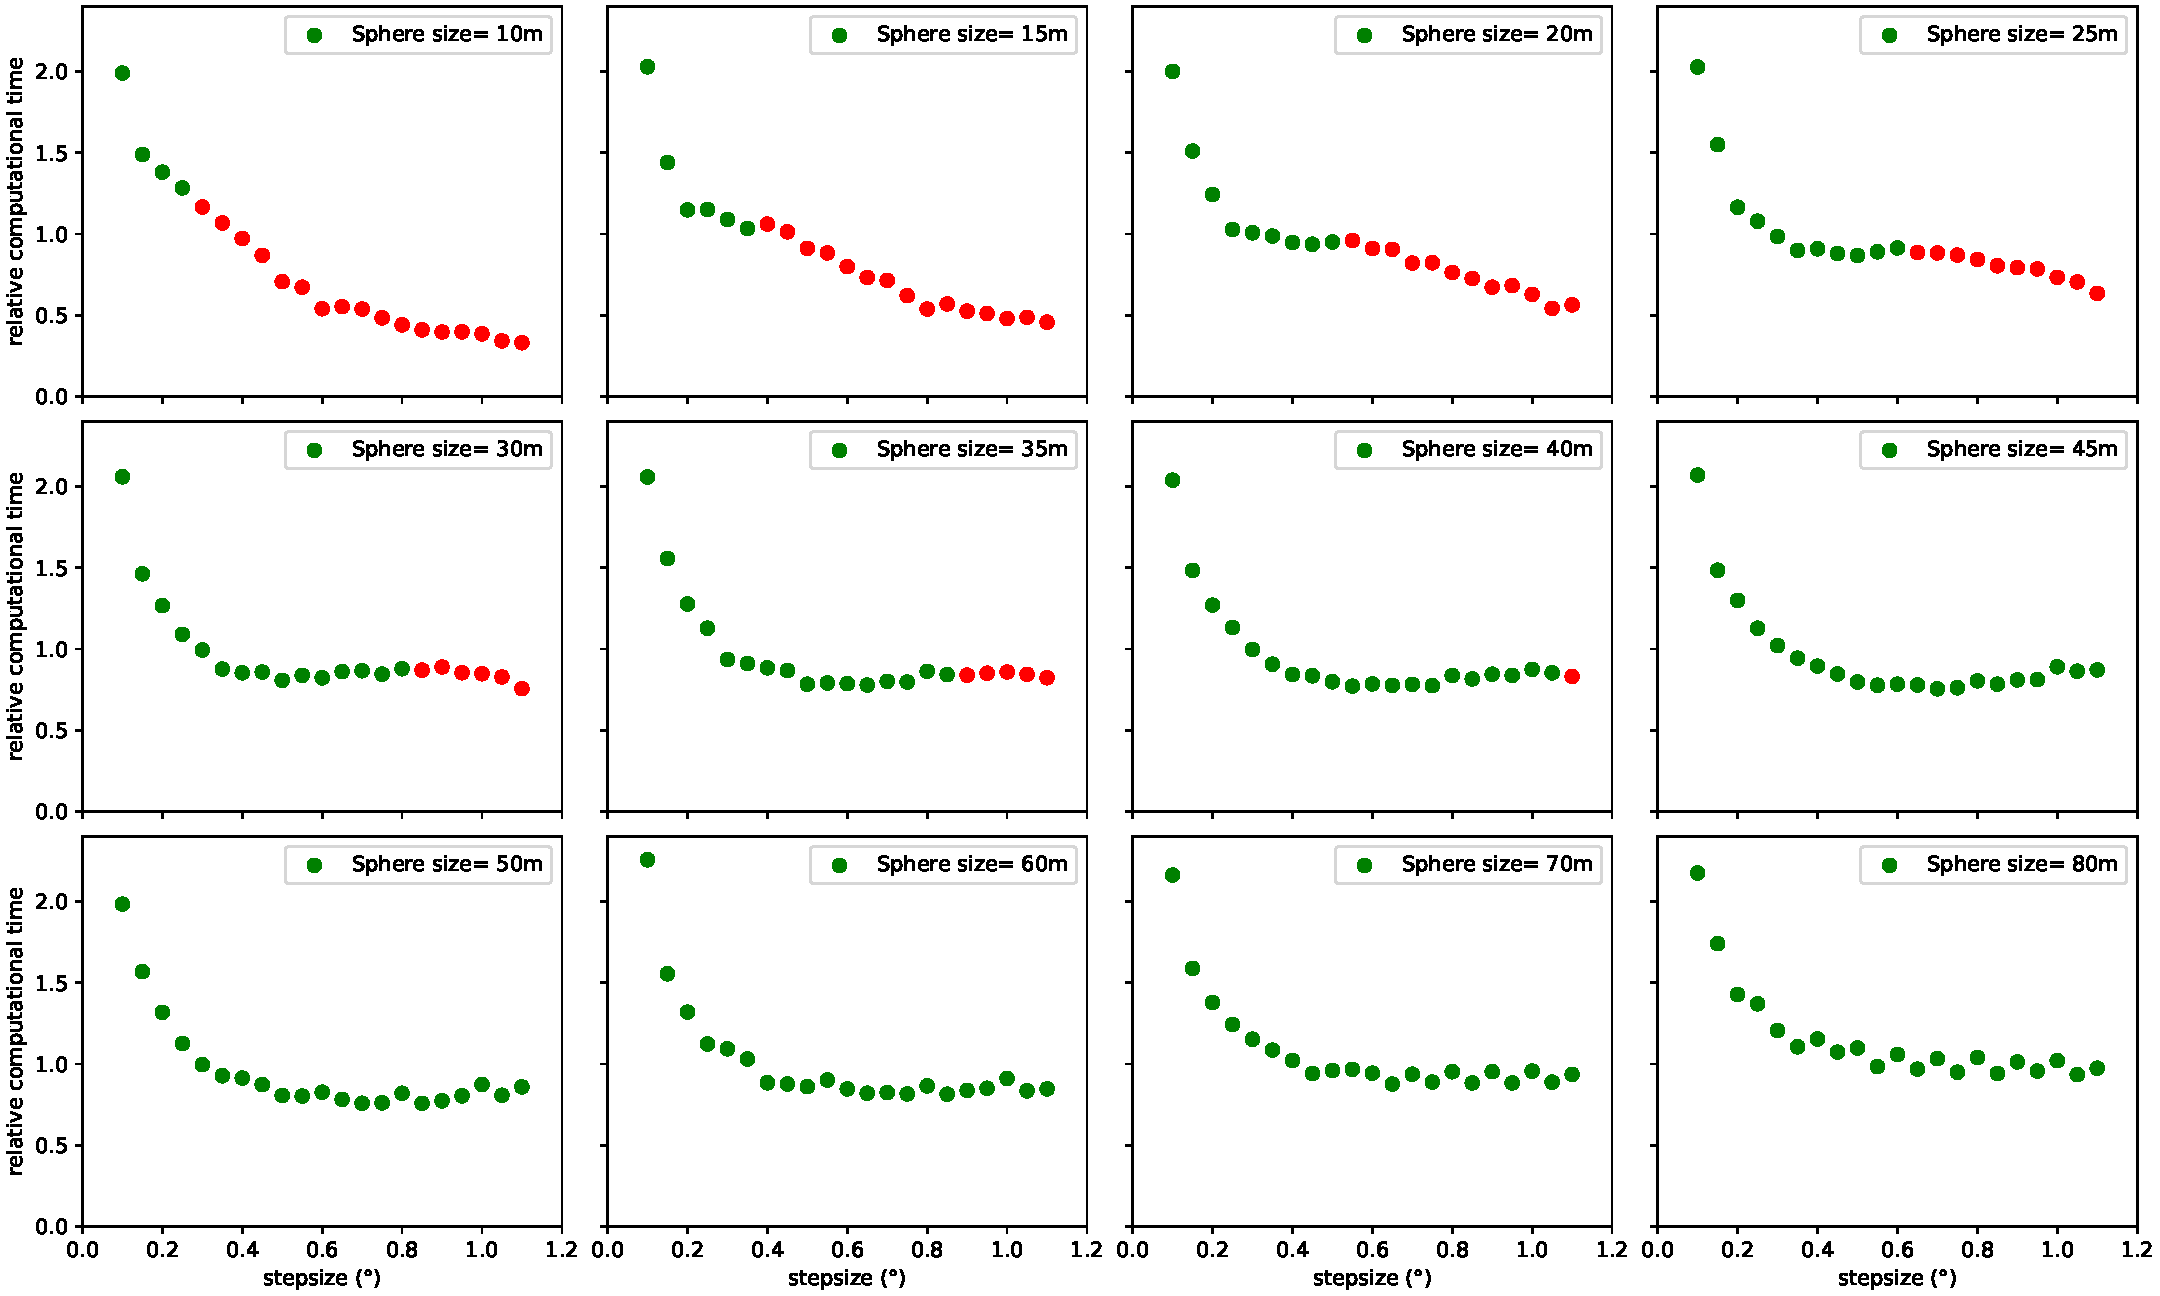
\includegraphics[width=\textwidth]{figures/subplotofallstepsphere.pdf}
	\caption{Variation in Sphere and angle step size with report on relative time.}
	\label{fig:SphereStepInfl}
\end{figure}

\begin{figure}
	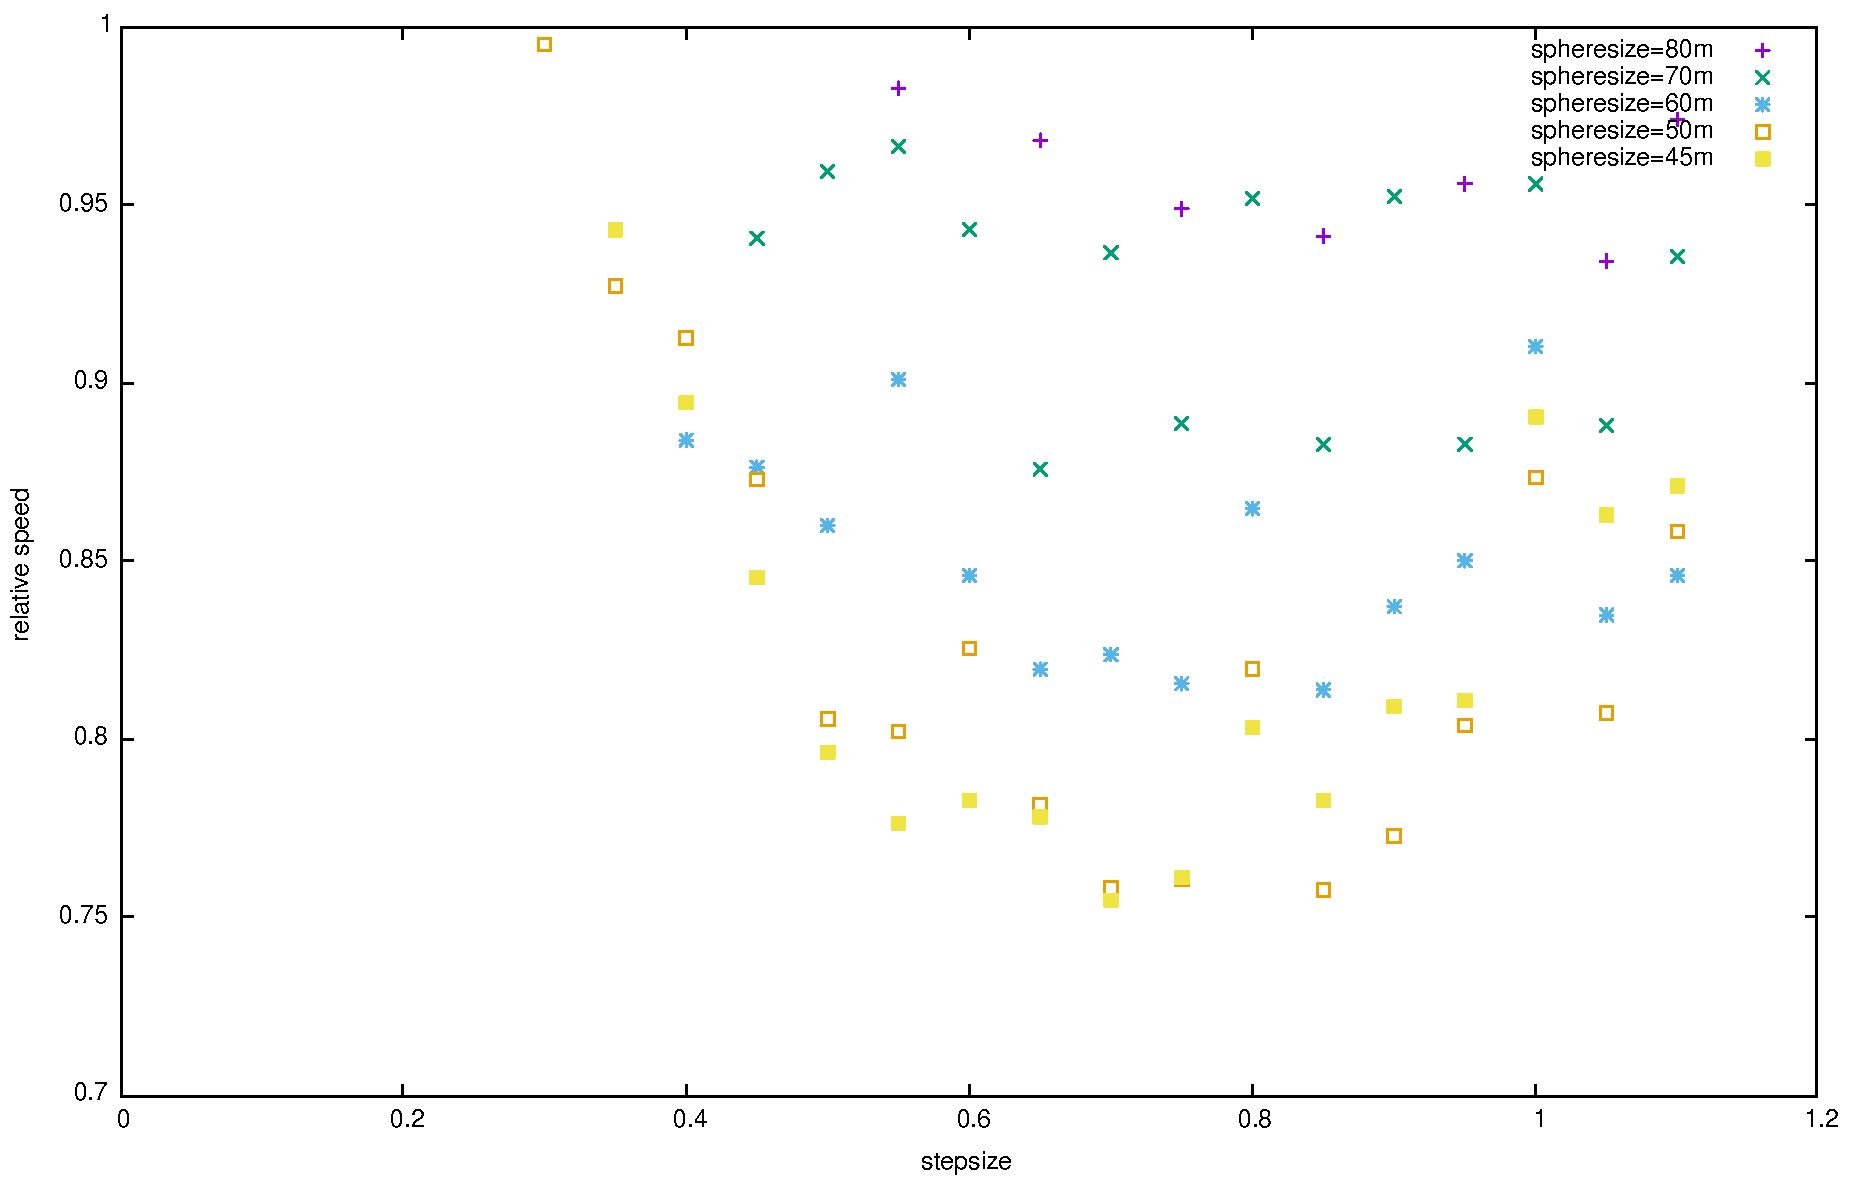
\includegraphics[width=\textwidth]{figures/SphereAndStepFinal.pdf}
	\caption{Green values in variation in sphere and angle step size with report on relative time.}
	\label{fig:SphereStepFinal}
\end{figure}

\chapter{Weather Balloon}
There are some changes that need to be made to the established hybrid minimizer, first off the air observer needs
to be hard removed as to make the simulation possible, second off the extra air observer needs to be removed that's additionally
defined for some reason and thirdly, the boundary behind the detector is now no longer vertical but horizontal.

Now having established this the first problem we'll consider is plane wave reconstruction of the original position, an example path to some of the sensors
is given in figure (...)
\begin{figure}
	\centering
	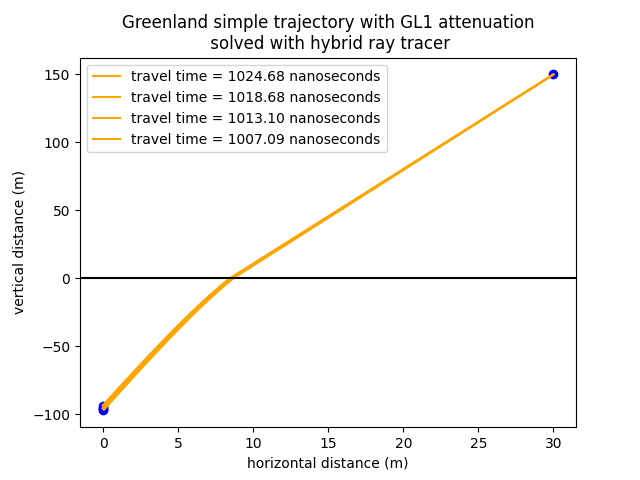
\includegraphics[width=0.7\textwidth]{weerballontraject.png}
\end{figure}
\begin{figure}
	\centering
	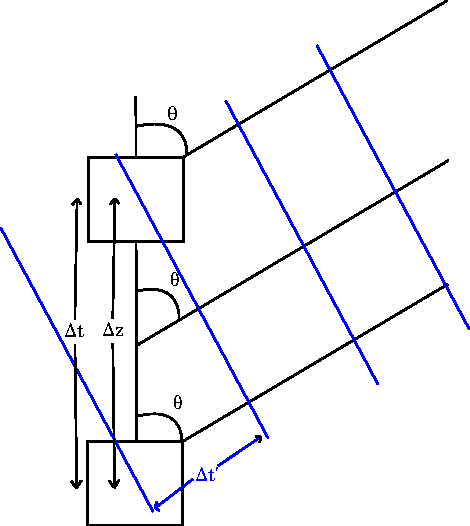
\includegraphics[width=0.7\textwidth]{planewave.pdf}
\end{figure}
\begin{equation}
	\Delta t' = \frac{m}{(m/s)} = (s/m)*m = v^{-1} * m = \frac{c}{n} \cos\theta \Delta z
\end{equation}
We take n to be 1.78 as 
%# from C. Deaconu, fit to data from Hawley '08, Alley '88
%# rho(z) = 917 - 602 * exp (-z/37.25), using n = 1 + 0.78 rho(z)/rho_0

\begin{equation}
	Correlation = \Delta t - \frac{\cos\theta \Delta z}{v}
\end{equation}

\begin{figure}
	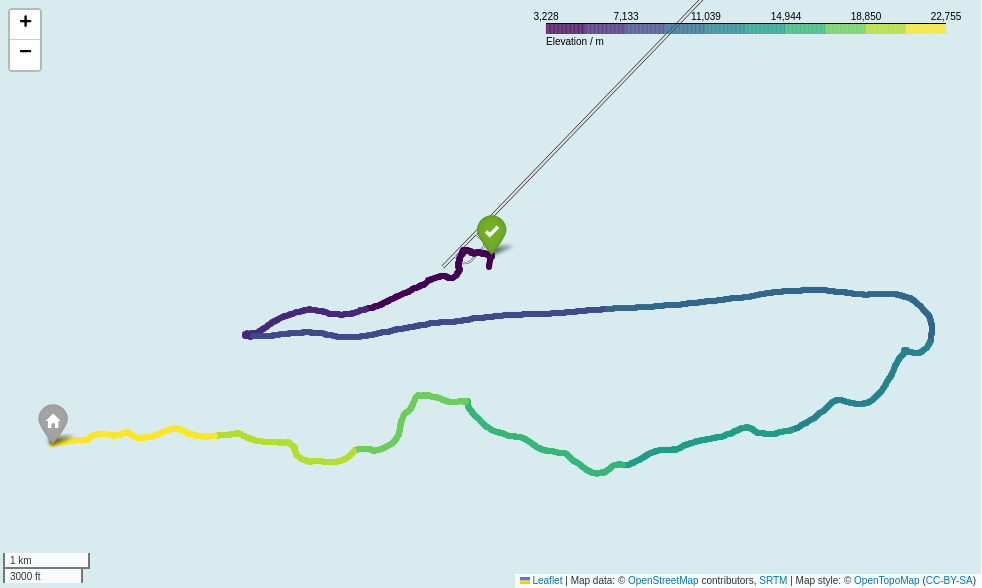
\includegraphics[width=\textwidth]{WeatherBalloonPath.png}
\end{figure}

\appendix
\chapter{Hybrid minimizer code}
\label{chapter: Hybrid minimizer code}
\begin{mintedbox}{python}
    def raytracer_hybrid_minimizer(self,n_reflections=0):
        """
        Uses RadioPropa to first find all the numerical ray tracing solutions between sphere x1 
        and sphere x2 for a big sphere. After which it uses the scipy optimize.minimize module
        to find the best path in these angle intervals. 
        Tracer does not work for reflective bottoms or secondary creation at the moment
        """

        try:
            X1 = self._X1 * (radiopropa.meter/units.meter)
            X2 = self._X2 * (radiopropa.meter/units.meter)
        except TypeError: 
            self.__logger.error('NoneType: start or endpoint not initialized')
            raise TypeError('NoneType: start or endpoint not initialized')
      
        def get_ray(theta,phi):
            ray_dir = hp.spherical_to_cartesian(theta,phi)
            if ray_dir.shape==(3,1): ray_dir = ray_dir.T[0] #doesn't always give the right shape
            source = radiopropa.Source()
            source.add(radiopropa.SourcePosition(radiopropa.Vector3d(*X1)))
            source.add(radiopropa.SourceDirection(radiopropa.Vector3d(*ray_dir)))
            ray = source.getCandidate()
            return ray

        def shoot_ray(theta):
            ray = get_ray(theta,phi_direct)
            sim.run(ray, True)
            return ray

        def cot(x):
            return 1/np.tan(x)

        def arccot(x):
            return np.arctan(-x) + np.pi/2

        def delta_z(cot_theta):
            theta = arccot(cot_theta)
            ray = shoot_ray(theta)
            ray_endpoint = self.get_path_candidate(ray)[-1]
            return (ray_endpoint-self._X2)[2]

        def delta_z_squared(cot_theta):
            return delta_z(cot_theta)**2

        def MinimizeAble(lower,upper):
            #This checks if there are 2 distinct regions, takes about 10^-6% of the total time
            if ((len(lower) == 2) and (len(upper)==2)):
                return ((lower[1] > upper[0]) and (lower[0] < upper[0]) and (lower[1] < upper[1]))
            else:
                return False

        LetsMinimize = False
 
        v = (self._X2 - self._X1)
        u = copy.deepcopy(v)
        u[2] = 0
        theta_direct, phi_direct = hp.cartesian_to_spherical(*v) # zenith and azimuth for the direct linear ray solution (radians)
        cherenkov_angle = np.arccos(1. / self._medium.get_index_of_refraction(self._X1))
        
        if np.linalg.norm(u) != 0:
            delta_theta = 2*abs(self.delta_theta_direct(dz=self._sphere_sizes[0]))
        else:
            delta_theta = self._step_sizes[0]/units.radian
            
        ## regions of theta with posible solutions (radians)
        launch_lower = [0]
        launch_upper = [theta_direct + delta_theta] # below theta_direct no solutions are possible without upward reflections

        if n_reflections > 0:
            if self.medium.reflection is None:
                self.__logger.error("a solution for {:d} reflection(s) off the bottom reflective layer is requested,"
                                    +"but ice model does not specify a reflective layer".format(n_reflections))
                raise AttributeError("a solution for {:d} reflection(s) off the bottom reflective layer is requested,"
                                    +"but ice model does not specify a reflective layer".format(n_reflections))
            else:
                z_refl = self._medium.reflection
                rho_channel = np.linalg.norm(u)
                if self._X2[2] > self._X1[2]: 
                    z_up = self._X2[2]
                    z_down = self._X1[2]
                else:
                    z_up = self._X1[2]
                    z_down = self._X2[2]
                rho_bottom = (rho_channel * (z_refl - z_down)) / (2*z_refl - z_up - z_down)
                alpha = np.arctan((z_down - z_refl)/rho_bottom)
                ## when reflection on the bottom are allowed, a initial region for theta from 180-alpha to 180 degrees is added
                launch_lower.append(((np.pi/2 + alpha) - 2*abs(self.delta_theta_bottom(dz=self._sphere_sizes[0], z_refl=z_refl) / units.radian)))
                launch_upper.append(np.pi)
        #we first do the same as in the iterative solver 
        for s,sphere_size in enumerate(self._sphere_sizes):

            sphere_size = sphere_size * (radiopropa.meter/units.meter)
            detected_rays = []
            results = []

            ##define module list for simulation
            sim = radiopropa.ModuleList()
            sim.add(radiopropa.PropagationCK(self._ice_model.get_scalar_field(), 1E-8, .001, 1.)) ## add propagation to module list
            for module in self._ice_model.get_modules().values(): 
                sim.add(module)
            sim.add(radiopropa.MaximumTrajectoryLength(self._max_traj_length * (radiopropa.meter/units.meter)))

            ## define observer for detection (channel)            
            obs = radiopropa.Observer()
            obs.setDeactivateOnDetection(True)
            channel = radiopropa.ObserverSurface(radiopropa.Sphere(radiopropa.Vector3d(*X2), sphere_size)) ## when making the radius larger than 2 meters, sometimes three solution times are found
             
            obs.add(channel)
            sim.add(obs)

            ## define observer for stopping simulation (boundaries)
            obs2 = radiopropa.Observer()
            obs2.setDeactivateOnDetection(True)
            w = (u / np.linalg.norm(u)) * 2*sphere_size
            boundary_behind_channel = radiopropa.ObserverSurface(radiopropa.Plane(radiopropa.Vector3d(*(X2 + w)), radiopropa.Vector3d(*w)))
            obs2.add(boundary_behind_channel)
            boundary_above_surface = radiopropa.ObserverSurface(radiopropa.Plane(radiopropa.Vector3d(0, 0, 1*radiopropa.meter), radiopropa.Vector3d(0, 0, 1)))
            obs2.add(boundary_above_surface)
            sim.add(obs2)
            
            #create total scanning range from the upper and lower thetas of the bundles
            step = self._step_zeniths[s] / units.radian
            theta_scanning_range = np.array([])
            for iL in range(len(launch_lower)):
                new_scanning_range = np.arange(launch_lower[iL], launch_upper[iL]+step, step)
                theta_scanning_range = np.concatenate((theta_scanning_range, new_scanning_range))

            for theta in theta_scanning_range:
                ray_dir = hp.spherical_to_cartesian(theta, phi_direct)
                
                def delta(ray_dir,shower_dir):
                    viewing = np.arccos(np.dot(shower_dir, ray_dir)) * units.radian
                    return viewing - cherenkov_angle

                if (self._shower_axis is None) or (abs(delta(ray_dir,self._shower_axis)) < self._cut_viewing_angle):
                    source = radiopropa.Source()
                    source.add(radiopropa.SourcePosition(radiopropa.Vector3d(*X1)))
                    source.add(radiopropa.SourceDirection(radiopropa.Vector3d(*ray_dir)))
                    sim.setShowProgress(True)
                    ray = source.getCandidate()
                    sim.run(ray, True)
                    
                    current_rays = [ray]
                    while len(current_rays) > 0:
                        next_rays = []
                        for ray in current_rays:
                            if channel.checkDetection(ray.get()) == radiopropa.DETECTED:
                                detected_rays.append(ray)
                                result = {}
                                if n_reflections == 0:
                                    result['reflection']=0
                                    result['reflection_case']=1
                                elif self._ice_model.get_modules()["bottom reflection"].get_times_reflectedoff(ray.get()) <= n_reflections: 
                                    result['reflection']=self._ice_model.get_modules()["bottom reflection"].get_times_reflectedoff(ray.get())
                                    result['reflection_case']=int(np.ceil(theta/np.deg2rad(90)))
                                results.append(result)
                            for secondary in ray.secondaries:
                                next_rays.append(secondary)
                        current_rays = next_rays
            #loop over previous rays to find the upper and lower theta of each bundle of rays
            #uses step, but because step is initialized after this loop this ios the previous step size as intented
            if len(detected_rays) > 0:
                launch_lower.clear()
                launch_upper.clear()
                launch_theta_prev = None
                for iDC,DC in enumerate(detected_rays):
                    launch_theta = DC.getLaunchVector().getTheta()/radiopropa.rad
                    if iDC == (len(detected_rays)-1) or iDC == 0:
                        if iDC == 0: 
                            launch_lower.append(launch_theta-step)
                        if iDC == (len(detected_rays)-1): 
                            launch_upper.append(launch_theta+step)
                    elif abs(launch_theta - launch_theta_prev) > 1.1*step: ##take 1.1 times the step to be sure the next ray is not in the bundle of the previous one
                        launch_upper.append(launch_theta_prev+step)
                        launch_lower.append(launch_theta-step)
                    else:
                        pass
                    launch_theta_prev = launch_theta
                isMinimizeAble = MinimizeAble(launch_lower,launch_upper) 
                #check if we have two distinct launch regions so we can minimize
                #accuracy is chosen above time duration, so this will take a while
                if isMinimizeAble and (s == 0): # speed hack: Only check on first iteration
                    LetsMinimize = True
                    break

            else:
                #if detected_rays is empty, no solutions where found and the tracer is terminated
                break

        if LetsMinimize:
            iterative = False
            ##define module list for simulation, this needs to be redone to get rid of the spherical observer
            sim = radiopropa.ModuleList()
            sim.add(radiopropa.PropagationCK(self._ice_model.get_scalar_field(), 1E-8, .001, 1.)) ## add propagation to module list
            for module in self._ice_model.get_modules().values():
                sim.add(module)
            sim.add(radiopropa.MaximumTrajectoryLength(self._max_traj_length*(radiopropa.meter/units.meter)))

            ## define observer for detection (channel)
            obs = radiopropa.Observer()
            obs.setDeactivateOnDetection(True)
            #a bigger normal value makes the calculation faster, a smaller one more precise
            #NormalScale = 2.5
            w = (u / np.linalg.norm(u)) #* NormalScale
            plane_channel = radiopropa.ObserverSurface(radiopropa.Plane(radiopropa.Vector3d(*X2), radiopropa.Vector3d(*w)))
            obs.add(plane_channel)
            sim.add(obs)

            # handy?
            boundary_above_surface = radiopropa.ObserverSurface(radiopropa.Plane(radiopropa.Vector3d(0, 0, 1*radiopropa.meter), radiopropa.Vector3d(0, 0, 1)))
            obs2.add(boundary_above_surface)
            sim.add(obs2)

            detected_rays = []
            detected_theta = []
            #we minimize the cotangens of the zenith to reflect the same resolution in z to the different angles (vertical vs horizontal)

            for i in range(len(launch_lower)):
                ll = launch_lower[i]
                lu = launch_upper[i]
                cotll = cot(ll)
                cotlu = cot(lu)
                InitGuess = cot((ll+lu)/2)
                if cotlu > cotll:
                    bounds = scipy.optimize.Bounds(lb=cotll, ub=cotlu, keep_feasible=False)
                else:
                    bounds = scipy.optimize.Bounds(lb=cotlu, ub=cotll, keep_feasible=False)

                root = optimize.minimize(delta_z_squared,x0=InitGuess,bounds=bounds,options={'xatol':self.__xtol**2,'fatol':self.__ztol**2},method='Nelder-Mead')
                theta = arccot(root.x)
                detected_theta.append(theta)
                detected_rays.append(shoot_ray(theta)) 

            self._rays = detected_rays
            self._results =  [{'reflection':0,'reflection_case':1} for ray in detected_rays]
            launch_bundles = None 
            self.__used_method = 'hybrid minimizer'
            return launch_bundles,iterative

        else:
            iterative = True
            self._rays = detected_rays
            self._results = results
            self.__used_method = 'iterator'
            launch_bundles = np.transpose([launch_lower, launch_upper])
            return launch_bundles,iterative
\end{mintedbox}


% =====================================================================
% End matter
% =====================================================================
\newpage
%----------------------------------------------------------------------------------------
%	REFERENCE LIST
%----------------------------------------------------------------------------------------
\bibliography{sources}
\bibliographystyle{plain}

\end{document}
